% ****** Start of file apssamp.tex ******
%
%   This file is part of the APS files in the REVTeX 4.2 distribution.
%   Version 4.2a of REVTeX, December 2014
%
%   Copyright (c) 2014 The American Physical Society.
%
%   See the REVTeX 4 README file for restrictions and more information.
%
% TeX'ing this file requires that you have AMS-LaTeX 2.0 installed
% as well as the rest of the prerequisites for REVTeX 4.2
%
% See the REVTeX 4 README file
% It also requires running BibTeX. The commands are as follows:
%
%  1)  latex apssamp.tex
%  2)  bibtex apssamp
%  3)  latex apssamp.tex
%  4)  latex apssamp.tex
%
\documentclass[%
 reprint,
%superscriptaddress,
%groupedaddress,
%unsortedaddress,
%runinaddress,
%frontmatterverbose, 
%preprint,
%preprintnumbers,
%nofootinbib,
%nobibnotes,
%bibnotes,
 amsmath,amssymb,
 aps,
%pra,
%prb,
%rmp,
%prstab,
%prstper,
%floatfix,
]{revtex4-2}

\usepackage{graphicx}% Include figure files
\usepackage{dcolumn}% Align table columns on decimal point
\usepackage{bm}% bold math
\usepackage{comment}
%\usepackage{hyperref}% add hypertext capabilities
%\usepackage[mathlines]{lineno}% Enable numbering of text and display math
%\linenumbers\relax % Commence numbering lines

%\usepackage[showframe,%Uncomment any one of the following lines to test 
%%scale=0.7, marginratio={1:1, 2:3}, ignoreall,% default settings
%%text={7in,10in},centering,
%%margin=1.5in,
%%total={6.5in,8.75in}, top=1.2in, left=0.9in, includefoot,
%%height=10in,a5paper,hmargin={3cm,0.8in},
%]{geometry}

\begin{document}

\preprint{PIRE-GEMADARC Internal Notes – Germanium Internal Amplification (GeIA)}

\title{PIRE-GEMADARC Internal Notes – Germanium Internal Amplification (GeIA):\\}% Force line breaks with \\
\thanks{}%

\author{Chih-Hsiang Yeh}
 \affiliation{Institute of Physics, Academic Sinica, Nangang, Taipei, Taiwan}%Lines break automatically or can be forced with \\
  \affiliation{Department of Physics, National Central University, Chungli, Taoyuan, Taiwan}%Lines break automatically or can be forced with \\


  \email{a9510130375@gmail.com}

\collaboration{PIRE-GEMADARC Collaboration}%\noaffiliation

\date{\today}% It is always \today, today,
             %  but any date may be explicitly specified

\begin{abstract}
To understand the solid-state physics emerging in the crystal for the germanium internal amplification at two conventional temperatures, which are liquid nitrogen temperature(77K) and liquid helium temperature(4K), some of the literature studies are completed with the content summarized in this note. 
\end{abstract}


%\keywords{Suggested keywords}%Use showkeys class option if keyword
                              %display desired
\maketitle

\tableofcontents

%%%%%%%%%%%%%%%%%%%%%%%%%%%%%%%%%%%%%%%%%%%%%%%%%%%%%%%%

\section{\label{sec:level1}Introduction}

Since some of the experiments, such as the low-mass WIMP search with $\chi N$ scattering, require the low-threshold detector for detecting the small amount of energy, the fundamental laws of internal amplification, which can be utilized for enlarging the signal directly, should be revealed for getting it to be manageable.\par
In 2000, two experts from Russian, who are the pioneers of our research, came up with the conceptual design about applying the high voltage on the Ge detector, along with the electron-hole pairs that can be enhanced within the avalanche region showing up in the crystal. Thereby, there are a bunch of experiments having an attempt to extend the idea and to see whether it can be worked out with the state-of-the-art technology in reality.\par
In our collaborations, two teams are realizing the notion under two conventional temperatures, which are 4K(USD) and 77K(THU). Under these two different temperatures, the phenomenon happening to the signal and noise in the crystal would be disparate. The studies are expected to carry out the difference between these two setups, and the advantage versus disadvantage in a variety of facets to them.\par
In the following sections, first, some of the basic knowledge related to the p-n junction would be conducted as the foundation of this research. Then, under these two temperatures mentioned previously, the internal amplification on the signal will be elaborated on. In parallel, as the signal is strengthened, the noise of the crystal could be unexpectedly magnified consequently. Dealing with the adversity of the high noise originating from three species of leakage currents in the crystal is the very next topic that should be addressed. After all, the signal-to-noise ratio is the ultimate criteria to compare between different setups.\par
At the end of the notes, first the calculation of the gain factor, which is based on the authentic electric field distribution in the P-type point contact(PPC) detector, would be regarded. Hereafter, in practical, because of the thorny problem on the dielectric breakdown, which is due to the tremendously high electric field and can sabotage the crystal intrinsically for both temperatures, the mechanism of that would be delivered to assess the crucial voltage on protecting the crystal from being destroyed. 

%%%%%%%%%%%%%%%%%%%%%%%%%%%%%%%%%%%%%%%%%%%%%%%%%%%%%%%%

\section{\label{sec:level2}Basic p-n junction}
Given the semiconductor containing the different types of impurity, two groups, including the n(electron-dominant) and p(hole-dominant) types, can be characterized. For any crystal containing both types of semiconductors, the properties of the p-n junction will occur. The phenomenon for it would be discussed as follows.\par
In Fig.\ref{PNPlot}, the typical p-n junction is illustrated. On the p-n junction, the electron-hole diffusion, as well as the attraction, will start emerging in the crystal. After the "dynamic" get balance, the neutral region called "the depletion region", which the stable electric field flows in, will show up. In the reverse-bias case, the higher the voltage, the larger the region it will be. In the end, the voltage should be enhanced to the one which can deplete the whole crystal, implying all electrons and holes in the crystal get equilibrium. Afterward, the application of this "neutral" crystal can start off.\par
\begin{figure}[h]
  \centering
  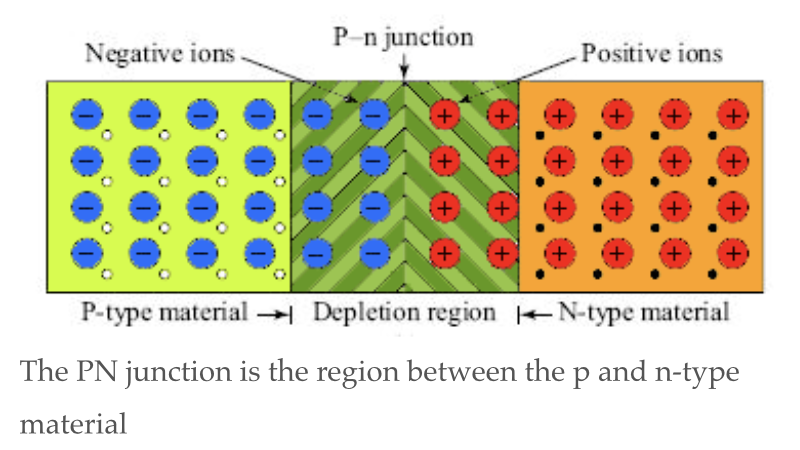
\includegraphics[width=0.35\textwidth]{/Users/yehchihhsiang/Desktop/Chronological_Results/2021-all/Education_Paper/SHEME/PN_Junction.png}
  \caption{The basic P-N Junction.}
  \label{PNPlot}
\end{figure}
Then, the voltage, which is applied to fully deplete the crystal, can be derived from the formula as follows:
\begin{equation}
\label{MFP}
x_{d} = \sqrt{ \frac{2\epsilon V_{d}}{q N_{a}}}
\end{equation}

$x_{d}$ is the depletion length as obtained from the crystal, $N_{a}$ is the impurity concentration, $V_{d}$ is the voltage solicited to do the task of the depletion.  After moving some of the parameters from right to left, then the depletion voltage can be demonstrated clearly:

\begin{equation}
\label{MFP}
V_{d} = \frac{x_{d}^{2}qN_{a}}{2\epsilon}
\end{equation}

In FIG.\ref{Depletion_Voltage}, the depletion voltage under the various temperatures for a detector with a length of 2.37cm is displayed. When the temperature becomes lower, the depletion voltage will be decreased.\par

\begin{figure}[h]
  \centering
  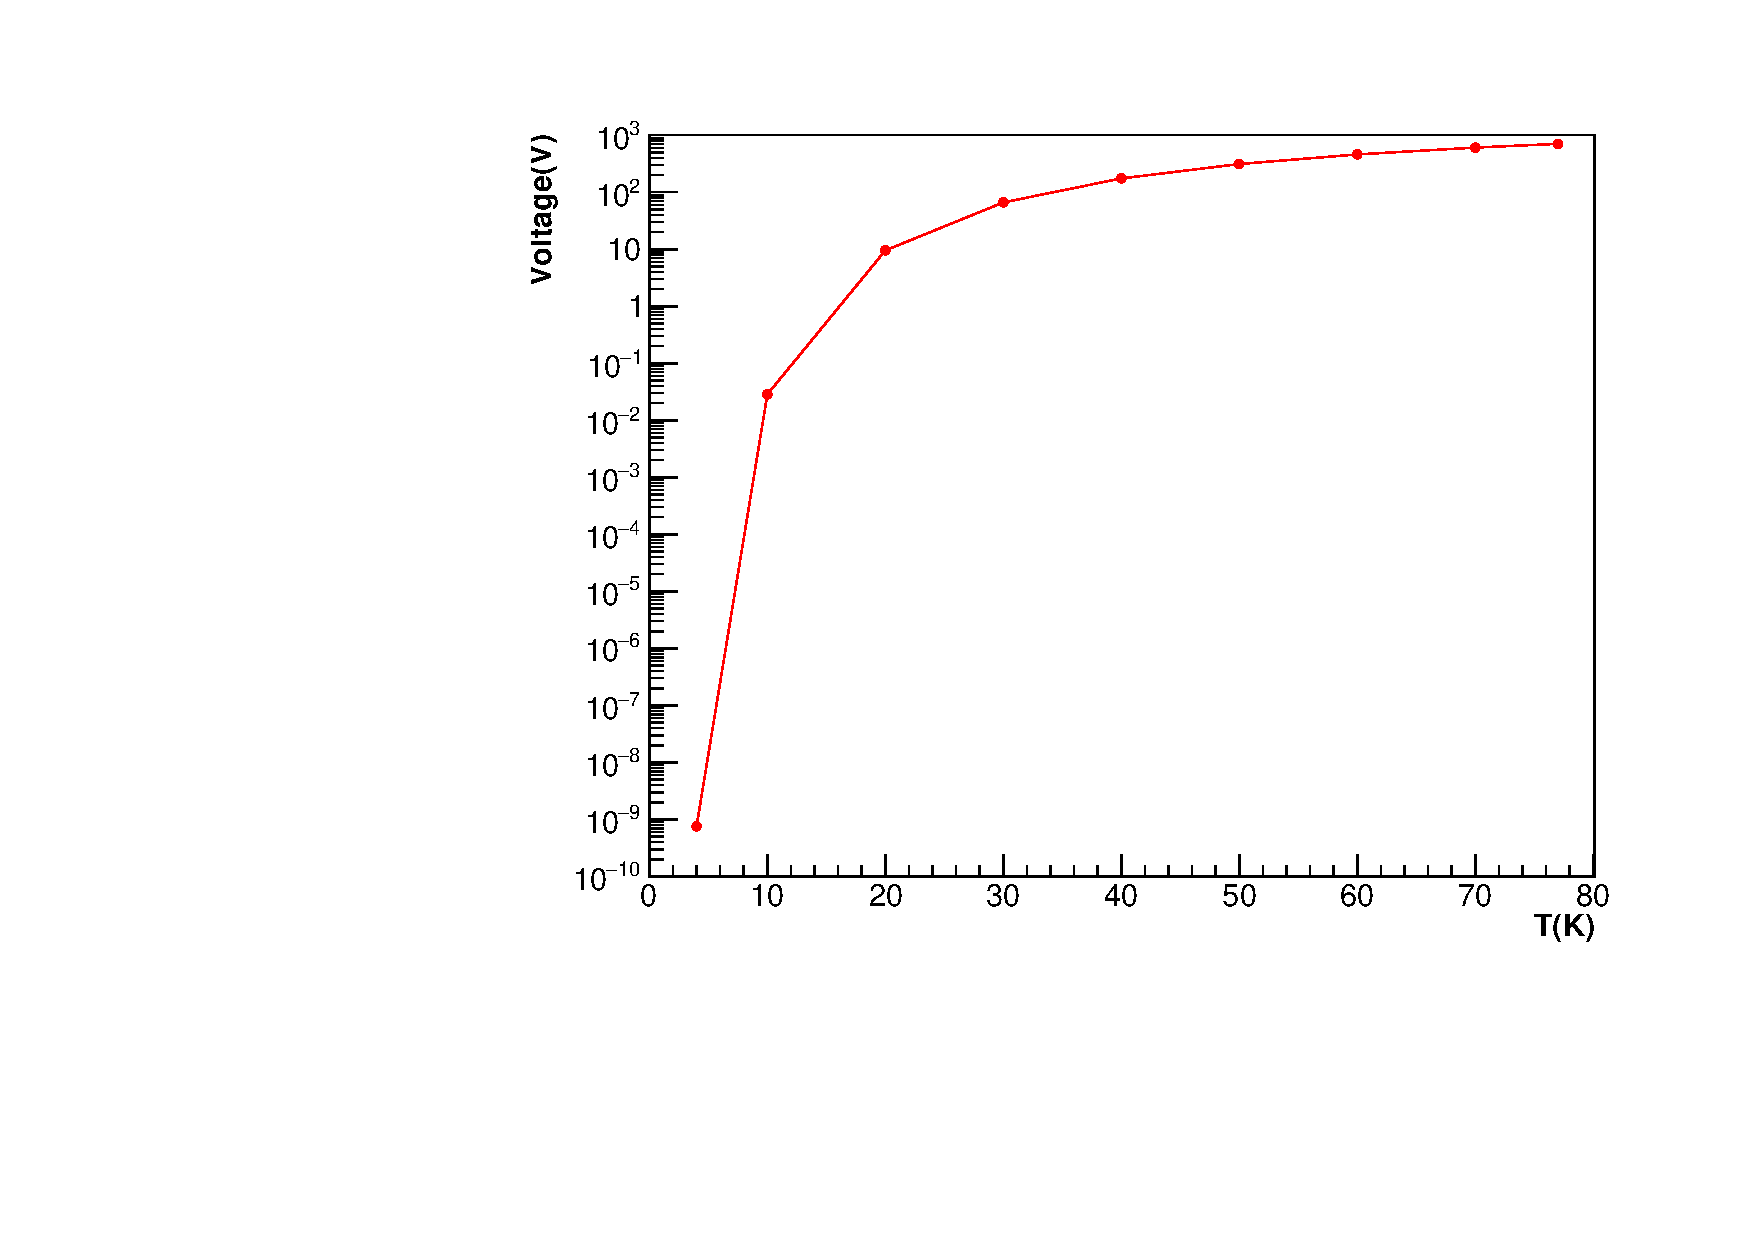
\includegraphics[width=0.35\textwidth]{/Users/yehchihhsiang/Desktop/Chronological_Results/2021-all/Education_Paper/Depletion_Length.pdf}
  \caption{The depletion voltage as a function of the temperature for the detector with the length equal to 2.37cm.}
  \label{Depletion_Voltage}
\end{figure}

If the details of it about the fundamental physics in semiconductor is desired, chapter7 and chapter8 of the book\cite{10.5555/1594006} are recommended.\par


%%%%%%%%%%%%%%%%%%%%%%%%%%%%%%%%%%%%%%%%%%%%%%%%%%%%%%%%

\section{\label{sec:level3}Signal Amplification}

\subsection{Necessary Parameters from "an electron":}
At the start, let us visualize "an electron", which is ionized by a WIMP, flowing in the crystal. Many necessary parameters must be acquired in advance from this electron to unfold our studies. All of them will be depicted in the following subsections.\par

%%%%%%%%%%%%%%%%%%%%%%%%%%%%%%%%%%%%%%%%%%%%%%%%%%%%%%%%
\subsubsection{$\text{Electrical Mobility($\mu$)}$}
From the definition of electrical mobility, which is as follows:
\begin{equation}
\label{Mobility}
\mu = \frac{V_{d} (1+\frac{E}{E_{sat}})}{E}
\end{equation}

$V_{d}$ is the velocity of the electron, and E is the electric field applied to the crystal.\par
The mobility is estimated by the formula above. Specially, since in our experiment, the ultra-high electric field is applied, the saturation phenomenon, referring to the situation that the velocity would be a constant when the electric field is beyond the critical one, can be obtained. In Fig.\ref{Electron_velocity}\cite{5}, when the electric field is upon $10^{4}\text{V/cm}$, which is also the critical electric field in calculating the ionization rate described in the latter section, the velocity of the electron is a constant for both temperatures.\par

\begin{figure}[h]
 \centering
 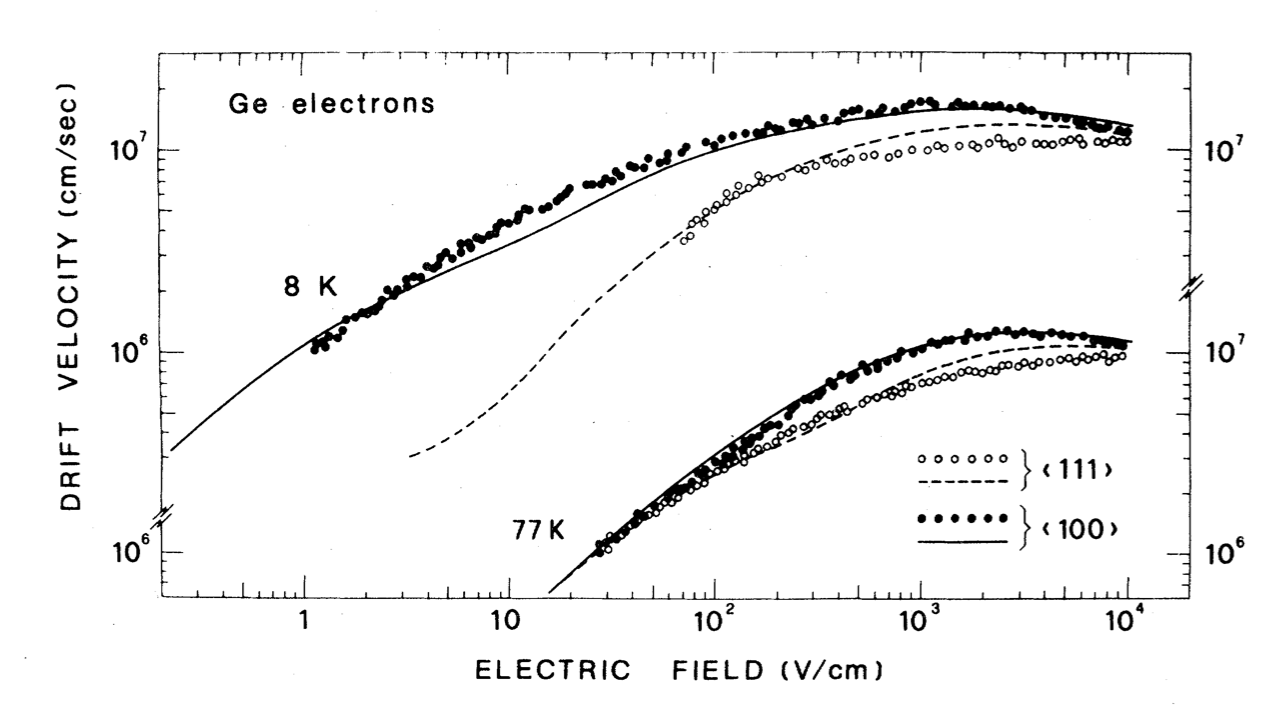
\includegraphics[width=0.5\textwidth]{SHEME/Electron_velocity.png}
 \caption{The drift velocity as a function of electric field is shown for the different temperatures.}
 \label{Electron_velocity}
\end{figure}
%%%%%%%%%%%%%%%%%%%%%%%%%%%%%%%%%%%%%%%%%%%%%%%%%%%%%%%%
\subsubsection{Effective mass(m*)}
Under the different temperatures, the effective conductivity masses are various. In Fig.\ref{effective_Mass_Relation}\cite{6}, the hole has the higher effective mass when the temperature is low. BTW, since there is no such study for Ge, Si study is taken as an instance to picture the tendency of the effective masses for the electron and the hole.  In our studies, the effective mass for the electron is simply set at m = 0.12m0 and for the hole, the effective mass is simply set at m=0.21m0.

\begin{figure}[h]
  \centering
  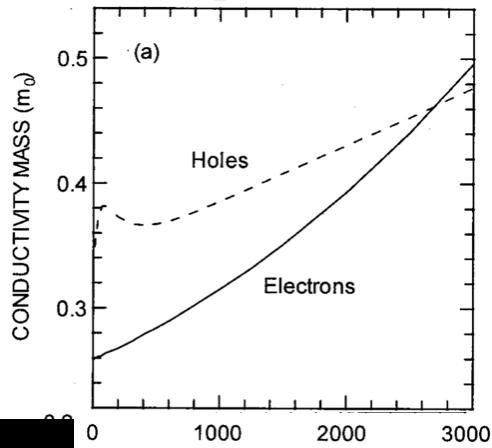
\includegraphics[width=0.35\textwidth]{SHEME/effective_Mass_Relation.png}
  \caption{The relation between the effective mass($m_{0}$) and the temperature(T) is demonstrated for both electron/hole in Si.}
  \label{effective_Mass_Relation}
\end{figure}

%%%%%%%%%%%%%%%%%%%%%%%%%%%%%%%%%%%%%%%%%%%%%%%%%%%%%%%%
\subsubsection{Relaxation Time($\tau$)}
The period of time that the electron can survive without bumping into another atom:\\ 
	
\begin{equation}
\tau = \frac{\mu \times m*}{e}
\end{equation}

e is the coulomb constant, $\mu$ is the mobility of the electron, and m* is the effective mass.\\
	
After acquainting the relaxation time, the next thing that should be figured out is the mean free path($\L$), which means how far the electron can go along without ramming with another atom in the crystal. The formula is as follows:\\
\begin{equation}
\label{MFP}
L = \tau \times V_{d}
\end{equation}

$V_{d}$ means the velocity of the electron, and $\tau$ is the relaxation time.\\

After all of the parameters are well-recognized in this section, those would be made use of in the next section for developing the theory of amplifying the signal.\\
%%%%%%%%%%%%%%%%%%%%%%%%%%%%%%%%%%%%%%%%%%%%%%%%%%%%%%%%
\subsection{Real beef: Ionization rate}
The ionization rate is defined as the following description: How many electrons/holes can be ionized within 1cm?\\

After depleting the crystal, next the relation between the ionization rate and the E(V/cm) can be brought to light. Based on the formulae (\ref{Ionization_Rate_1}),(\ref{Ionization_Rate_2}) and (\ref{Ionization_Rate_3}) from paper\cite{2}, the ionization rate can be decided by exploiting the mean free path(L), electric field(E(x)) and ionization energy(U) of the material, 
\begin{equation}\label{Ionization_Rate_1}
\alpha_{s} = \frac{a_{s}}{z} exp(-\frac{b_{s}}{E(x)})
\end{equation}
 \begin{equation}\label{Ionization_Rate_2}
z(x) = 1 + \frac{b_{n}}{E(x)} exp(-\frac{b_{n}}{E(x)}) + \frac{b_{p}}{E(x)} exp(-\frac{b_{p}}{E(x)})
\end{equation}
 \begin{equation}\label{Ionization_Rate_3}
a_{s} = \frac{1}{L_{s}}, b_{s} = \frac{U_{s}}{qL_{s}}, s = ( p , n ) type
\end{equation}

$\alpha_{s}$ means the Ionization rate, E(x) is the electric field distributing in the crystal, $L_{s}$ is the mean free path\footnote{Since the value of the mean free path is set a constant for a given temperature in the pioneer paper, we use 490nm for 77K and  }, and $U_{s}$ means the Ionization energy, which is set to be 3eV as measured in this paper\cite{Wei:2016xbw}.\\

The FIG.\ref{Ionization_rate} can be framed by employing the formulae introduced above. From this scheme, there are three important pieces of information that can be concluded:

\begin{figure}[h]
  \centering
  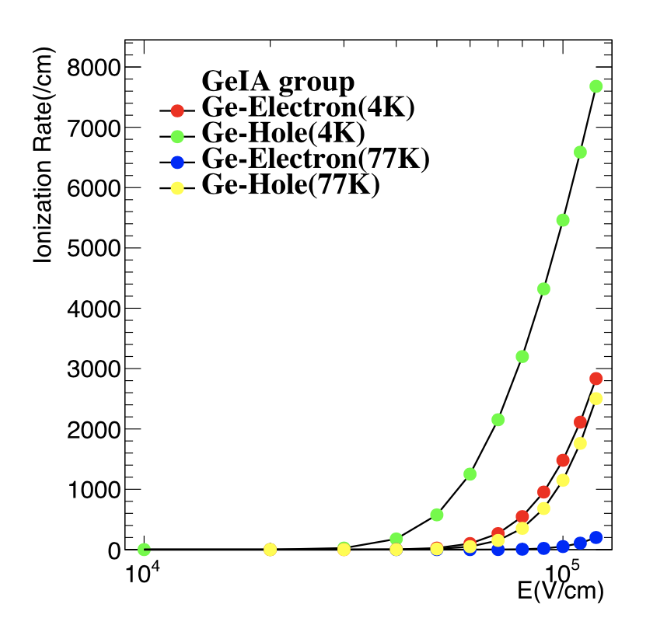
\includegraphics[width=0.35\textwidth]{SHEME/Ionization_Rate.png}
  \caption{The ionization rates for both electron and hole under both 4K and 77K.}
  \label{Ionization_rate}
\end{figure}

\begin{enumerate}
	\item Critical E=$10^{4}$ V/cm
	\item The significant difference between e/h cases is the effective mass under such high electric field at the same T.
	\item Hole can give us more signal under 4K.
\end{enumerate}
%%%%%%%%%%%%%%%%%%%%%%%%%%%%%%%%%%%%%%%%%%%%%%%%%%%%%%%%

\subsection{Pioneer: Russian investigation[2000]}
In light of the paper\cite{1}, the conceptual design on the coaxial detector HPGe, which is displayed in FIG.\ref{GeIA_Pioneer}, is provided. In order to estimate the gain factor, which is a criteria for the performance of the detector as described in the end of this note, the electric field distributing in the detector should be recognized beforehand. The distributions in the strip detector can be illustrated with the impurity concentration as the following formula:\\

\begin{equation}
\label{Electric_field}
E(r) = \frac{Ne}{2\epsilon}r-\frac{V+\frac{Ne}{4\epsilon}(R_{2}^{2}-R_{1}^{2})}{r \ln(\frac{R_{2}}{R_{1}})}
\end{equation}

where N is the impurity concentration, e is the electron charge, 􏰊$\epsilon$ is the dielectric constant of the germanium, $R_{2}$ and $R_{1}$ are the radii of the cathode and the anode, and V is the applied voltage.
\begin{figure}[h]
 \centering
 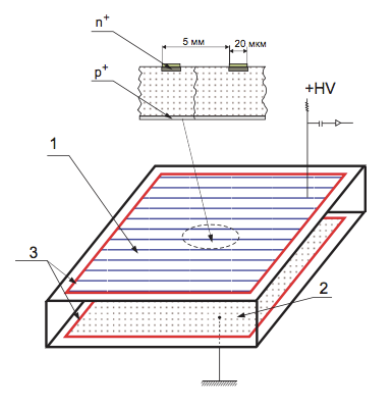
\includegraphics[width=0.35\textwidth]{SHEME/GeIA_Pioneer.png}
 \caption{Germanium detector with an internal amplification (schematic view): (1) anode strips, (2) cathode, and (3) guard electrodes. The scheme of n+ and p+ layers is shown in the upper part of the figure.}
 \label{GeIA_Pioneer}
\end{figure}


According to FIG.\ref{Ionization_rate}, when the electric field is higher than $10^{4}$(V/cm), the electron will be increased as the function of the electric field. As a result of that, after the electric fields with the different impurity concentrations are demonstrated in FIG.\ref{Avalanche_Reach_Through}\cite{1}, which is based on the calculation by the formula(\ref{Electric_field}), two regions can be separated with this critical electric field. 

\begin{enumerate}
	\item Avalanche region: When the electric field is above $10^{4}$(V/cm), the avalanche effect will emerge, subsequently, the signal will be amplified. 
	\item Reach-through region: If the electric field is below the critical one, then the electron/hole will just go through normally without any effect.
\end{enumerate}


\begin{figure}[h]
 \centering
 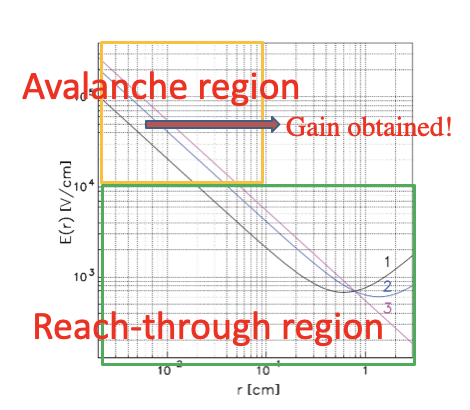
\includegraphics[width=0.35\textwidth]{SHEME/Avalanche_Reach_Through.png}
 \caption{The electric field as a function of the distance from the strip in FIG.\ref{GeIA_Pioneer} with the different impurities. The numbers above the lines mean the different impurities: (1)$10^{10} cm^{-3}$, (2)4 $\times 10^{9} cm^{-3}$ and (3) 0 $cm^{-3}$}
 \label{Avalanche_Reach_Through}
\end{figure}

These studies give out a clue that the detector can be devised to yield the amplification for the signal with the electric field above a certain level.
%%%%%%%%%%%%%%%%%%%%%%%%%%%%%%%%%%%%%%%%%%%%%%%%%%%%%%%%

\section{\label{sec:level3}Noise in the Crystal}
Unfortunately, the noise in the crystal is inevitable. The genres of the noise in the crystal should be characterized as the criteria of the limitation of measuring the lowest mass for dark matter theoretically. 
There are three sorts of noise in the crystal, encompassing the bulk leakage current, the contact leakage current, and the surface leakage current. In the following paragraph, all of them are described individually.\\

\subsection{Bulk leakage current}
Due to the thermal fluctuation, the electrons from the bulk(purity, such as Ge) material will be ionized possibly. Fortunately, the level of this noise can be ignored below 77K. The associated information is well-written in the formula(\ref{bulk_leakage_current})\cite{doi:10.1063/1.4953147}:
\begin{equation}\label{bulk_leakage_current}
I = A e^{\frac{-E_{\text{Ge Band}}}{2k_{B}T}}*q*\frac{1}{t}
\end{equation}
A is the intrinsic concentration, $E_{\text{Ge Band}}$ is the band gap of Ge, q is the coulomb constant, T is the  temperature(K), and t is the period of the time the electron/hole would come to the detector.
\subsection{Contact leakage current}
Because of 
\begin{enumerate}
	\item Barrier between the semi-metal connection
	\item Thermal fluctuation
\end{enumerate}

There is a possibility that the electron in the conductive band could leap into the metal, leading to the dark current which is unwanted.\\

In Fig.\ref{Contact_Leakage_2}\cite{Wei_2018}, which is the measurement from USD, gives out the thread about the scale of the contact leakage current at 100K is around $5 \times 10^{-10}A/cm^{2}$. Compared with our result, the Fig.\ref{Contact_Leakage_1}\cite{LOOKER2015138}, which is demonstrated by other group with the a-Ge detector, also has the similar results at 100K. Upon the usage of FIG.\ref{Contact_Leakage_1}, the contact leakage current under 77K, which is around $5 \times 10^{-16} A/cm^{2}$. can be extrapolated.\\

\begin{figure}[h]
  \centering
  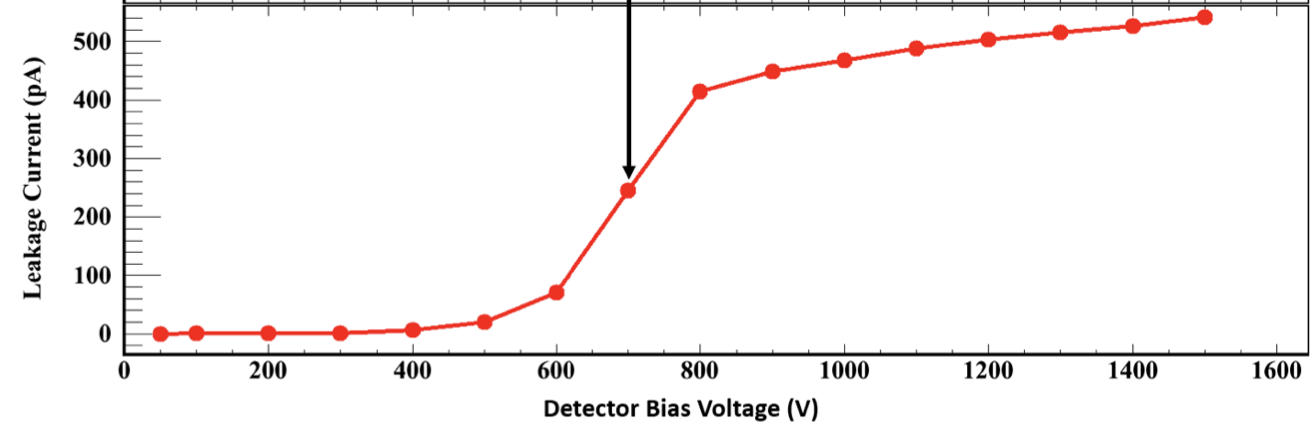
\includegraphics[width=0.5\textwidth]{SHEME/Contact_Leakage_2.png}
  \caption{The determination of full depletion voltage for detector USD-L01 using  I-V measurements at 100 K.}
  \label{Contact_Leakage_2}
\end{figure}

\begin{figure}[h]
  \centering
  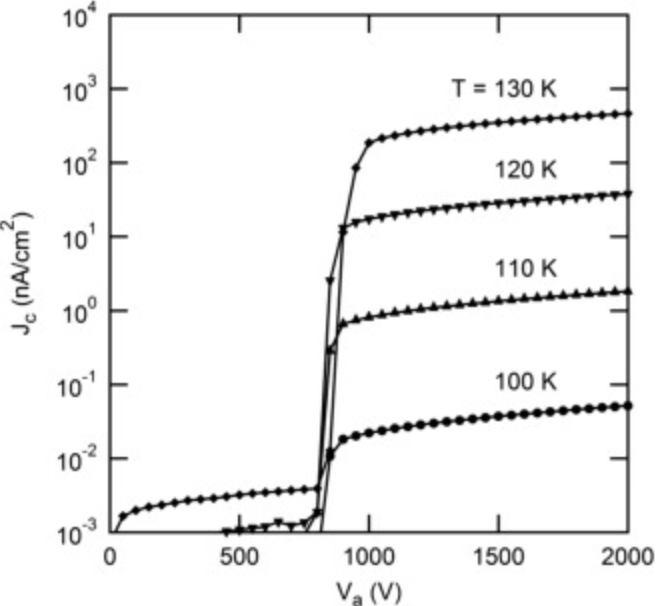
\includegraphics[width=0.35\textwidth]{SHEME/Contact_Leakage_1.png}
  \caption{Measured center contact leakage current density plotted as a function of bias voltage at various temperatures for an a-Ge/HPGe/a-Ge detector}
  \label{Contact_Leakage_1}
\end{figure}


The fundamental physics is "Schottky effect", which is a kind of the thermal emission. The simplified formula can be expressed with the "Richardson's law" as follows:\\ 
\begin{equation}
I \propto T^{2} e^{\frac{W}{k_{B}T}}
\end{equation}
$E_{\text{Ge Band}}$  is the band gap of Ge, q is the coulomb constant, T is the temperature(K), W is the work function of the material, and A is the measured constant.\\

The detail of this mechanism is compiled in the book\cite{10.5555/1203347}. Basically, it is a Metal-Semiconductor junction problem, which is a very big topic authentically and the chapter 10, 11 of book\cite{10.5555/1203347}(Strongly recommended!) and chapter 6 and 7 of book\cite{MILNES1972171} are recommended to acquire more detail on the related topic.\\

\subsection{Surface leakage current}
It depends on the quality of the crystal. By and large, lowering the temperature can help get rid of the noise.\\ 

There are two papers depicting the measurement of the surface leakage current for Ge. Please look at Fig.\ref{Surface_Leakage_Current}\cite{5871995}, which shows the surface leakage current from InAs Avalanche Photodiodes. Although this is not for Ge, it gives us a hint on the scale of the semiconductors. The points($\blacksquare$) can be expanded in the figure to predict the surface leakage current under more lower temperatures. The extremely low surface leakage current can be inferred in this paradigm under the low temperature.\\ 

Currently, the new results of a-Ge for the surface leakage current from USD are published. Amazingly, In FIG.\ref{Surface_Leakage_Current_2}\cite{Bhattarai:2020tal}, the leakage current is projected down to the temperature at 4K, and the considerably low leakage current is illustrated at the very low temperature, leading to the feasibility of detecting the low-mass dark matter.\\

\begin{figure}[h]
  \centering
  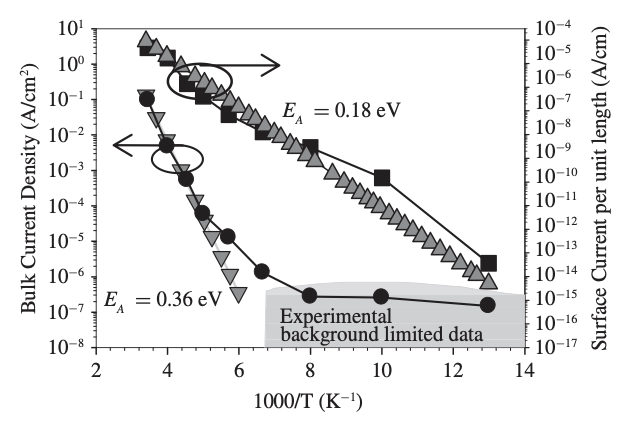
\includegraphics[width=0.4\textwidth]{SHEME/Surface_Leakage_Current.png}
  \caption{The surface leakage current, which is remarked by ($\blacksquare$), is measured with the InAs Avalanche Photodiodes.}
  \label{Surface_Leakage_Current}
\end{figure}

\begin{figure}[h]
  \centering
  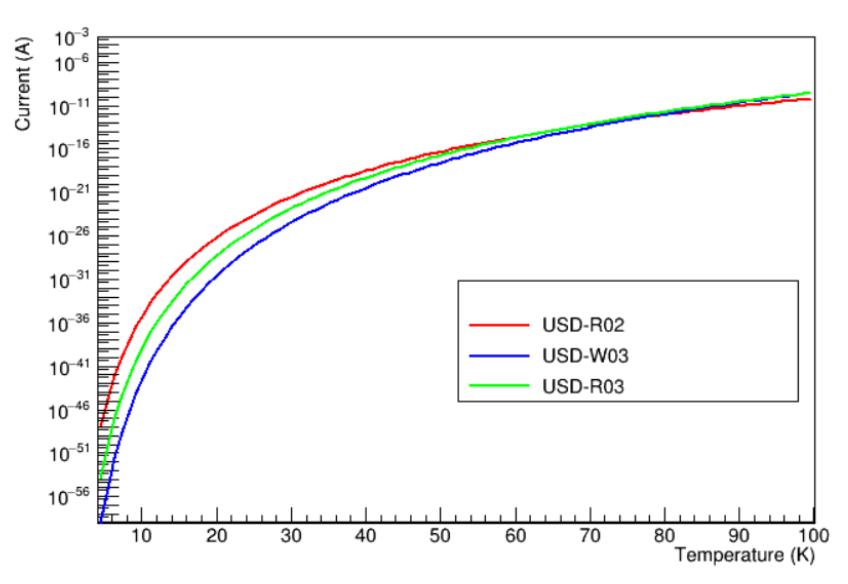
\includegraphics[width=0.4\textwidth]{SHEME/Surface_Leakage_Current_2.png}
  \caption{Projected variation of the surface leakage current with temperature for a PPC detector using the parameters obtained for the a-Ge used in detectors USD-R03, USD-R02 and USD-WO3.
.}
  \label{Surface_Leakage_Current_2}
\end{figure}


$$\\
$$\\
\subsection{Summary for three currents}

In FIG.\ref{Leakage_Current_Summary}, the chart for summarizing these three currents under the saturation circumstance are displayed. Overall, the surface leakage current is the severe conundrum for any temperature. At 77K, the contact leakage current is competitive with the surface leakage current, as their numbers are very close to each other.  At 4K, surprisingly, the surface leakage current surpasses all others overwhelmingly. \\

\begin{figure}[h]
  \centering
  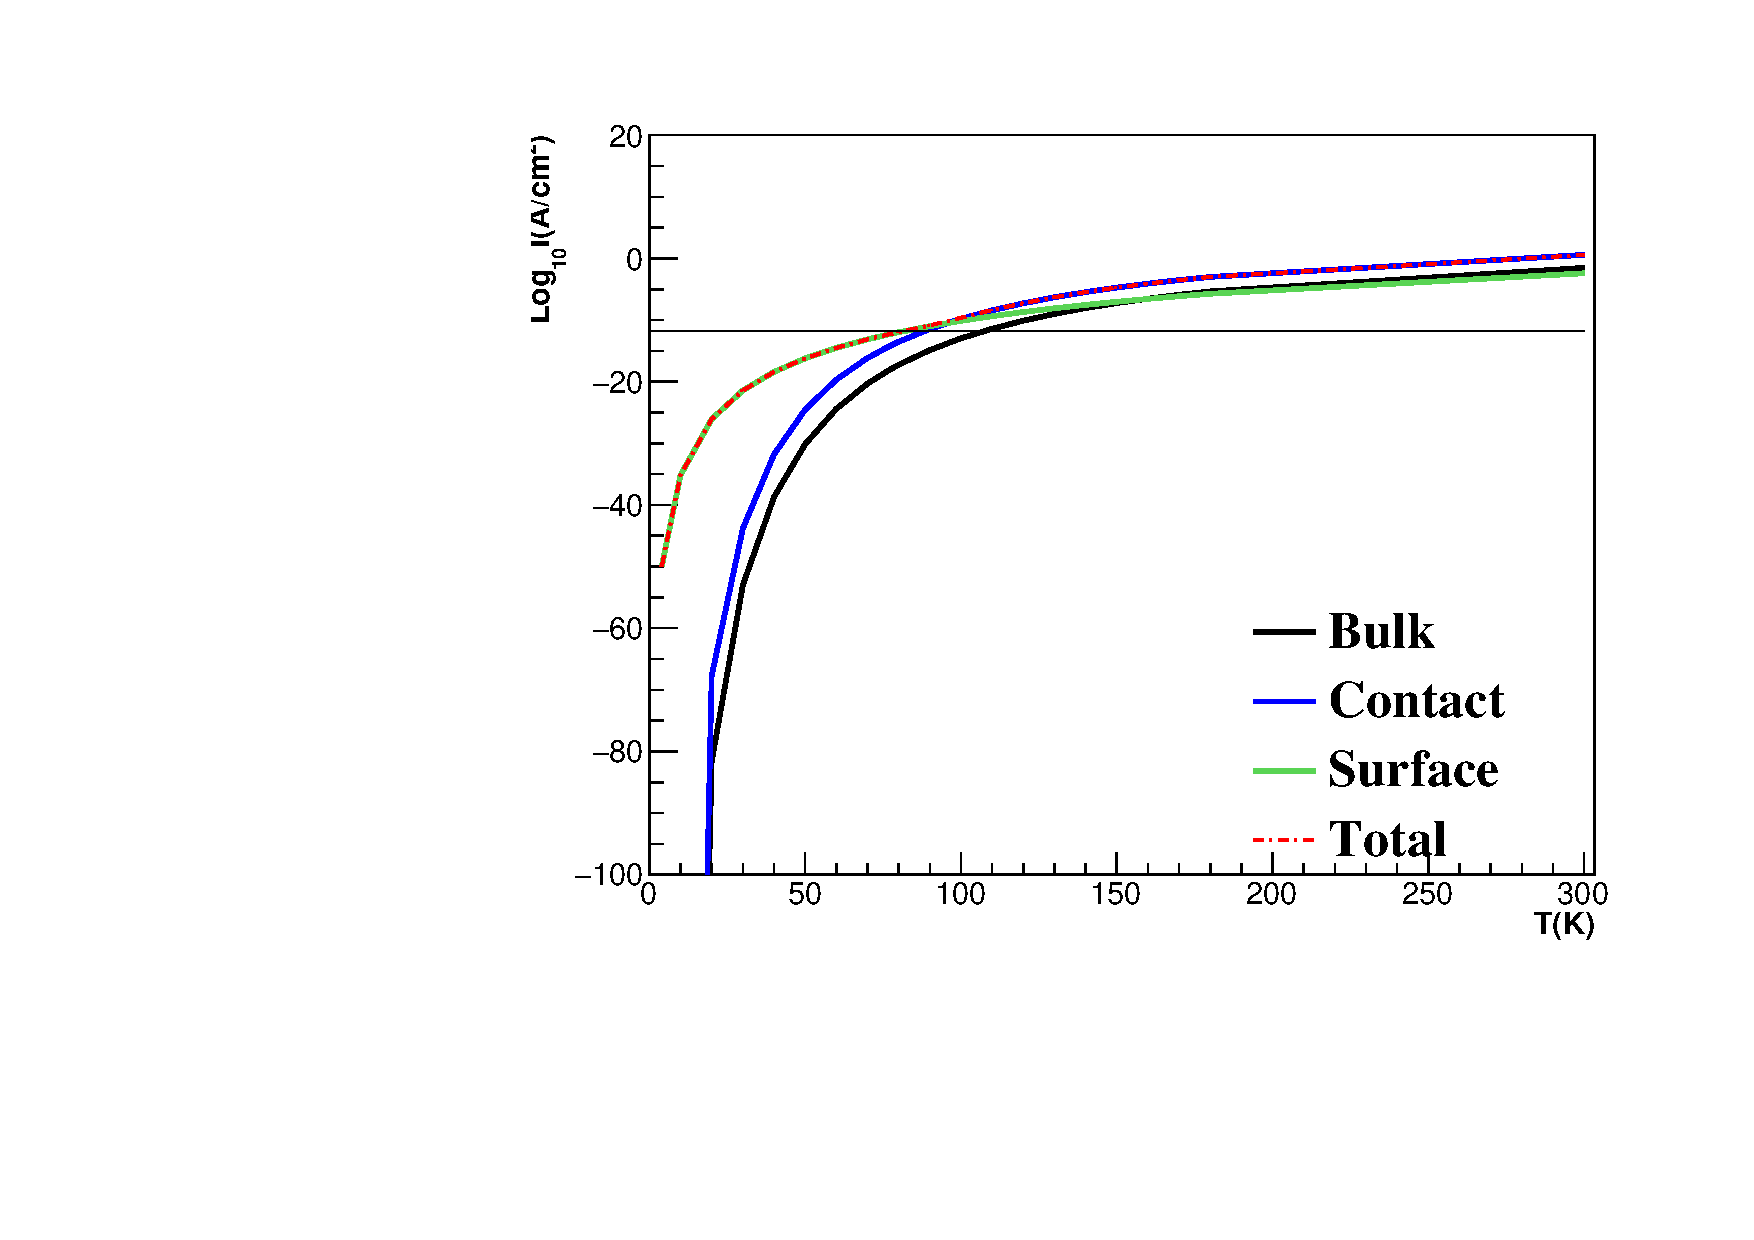
\includegraphics[width=0.4\textwidth]{Leakage_Current_Summary.pdf}
  \caption{The leakage current as a function of the temperature for three types of leakage currents.}
  \label{Leakage_Current_Summary}
\end{figure}

\section{Performance for the Detector}
In this section, the performance of the detector is expected to be projected under both temperatures with the information at hand. 

\subsection{Gain}
The gain factor can be estimated with two parameters, including the electric field and the ionization rate. Given the geometry of the detector, the gain factor can be obtained:\\
\begin{equation}
G = \int \alpha_{s}(E) \times E(r) dr
\end{equation}

In order to estimate the gain factor for the detector at both temperatures, the electric field distribution, which is geometry-dependent, should be identified in the different shapes of the detectors.\\

Since the distributions of the electric field under two temperatures are near the same under the same voltage in the strip detector, which can be carried out with the formula(\ref{Electric_field}), the same pattern is assumed to be the tenet for the P-type point contact(PPC) detector, meaning that in our case, the electric field distribution is voltage-dependent and temperature-independent.\\ 

The electric field distribution in FIG\ref{Electric_Field_PPC}, which is given by the Akash report(2018-08-09), is utilized in these studies. Since there is no direct result for the electric field under a bunch of the voltages in the PPC detector, the extrapolation with the strip detector is implemented. The relation in the following formula can be employed to predict the electric field under the different voltage in the PPC detector: \\

\begin{figure}[h]
  \centering
  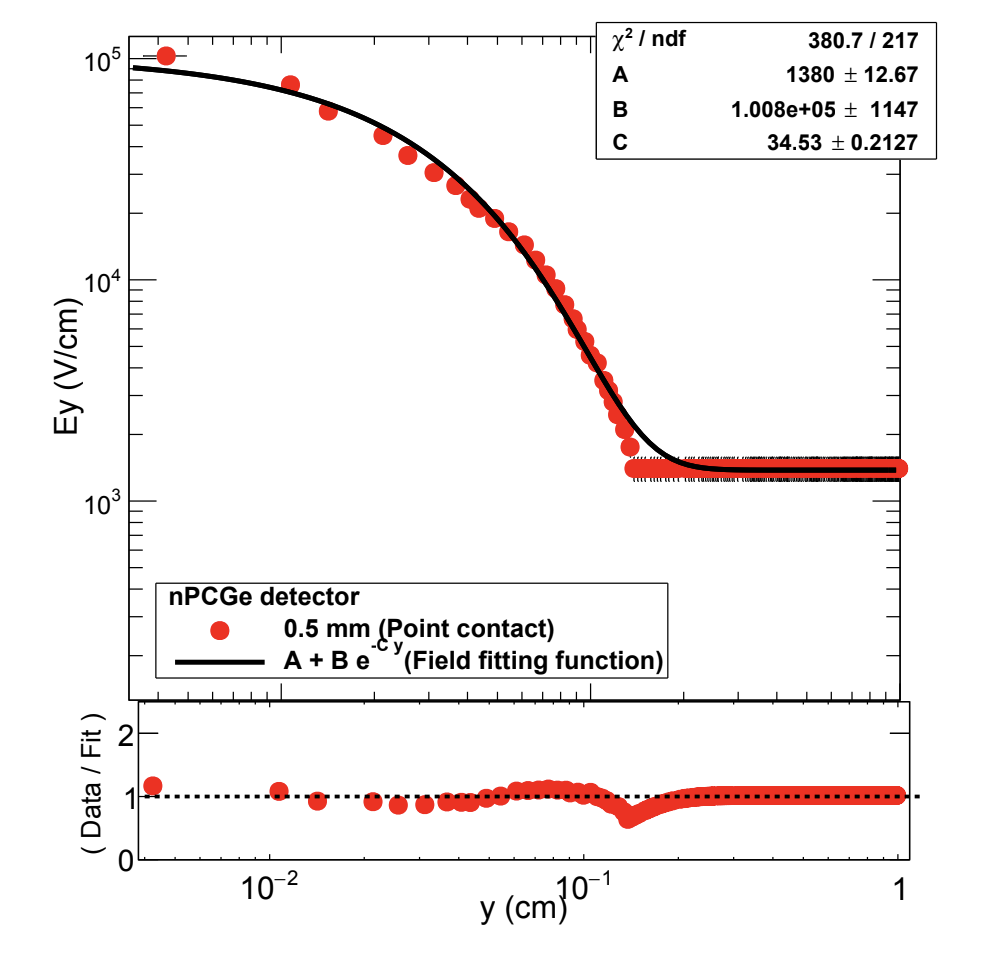
\includegraphics[width=0.4\textwidth]{Electric_Field_PPC.png}
  \caption{The electric field distribution as a function of the radius.}
  \label{Electric_Field_PPC}
\end{figure}

\begin{equation}\label{bulk_leakage_current}
\text{Strip detector }\frac{E_{3500V}}{E_{xV}}= \text{PPC detector} \frac{E_{3500V}}{E_{xV}}
\end{equation}

x is the desired voltage.\\

After fully plotting out the electric field distribution in the PPC detector, incorporating with the ionization rate portrayed in FIG.\ref{Ionization_rate}, the predictions for gains under both temperatures can be 
yielded as demonstrated in FIG.\ref{Gain}. The small conclusion framed by this plot is that the lower the temperature we use, the lower the voltage should be applied to the crystal for achieving the same gain below 1000. Furthermore, after zooming in the region from G=1 to G=3, which is exhibited in FIG.\ref{Gain_Zoom}, the clear point at 3500V for initiating the generation of the internal amplification can be observed under 77K. At 4K,1500V is claimed to kick off the process of the internal amplification.\\

Albeit the lower voltage is required to attain the same gain at the lower temperature, the breakdown phenomenon, which can arise to havoc the crystal as the applied voltage exceeds the critical one, so called "breakdown voltage", should be well recognized for preventing our detector from being exterminated. 

\begin{figure}[h]
  \centering
  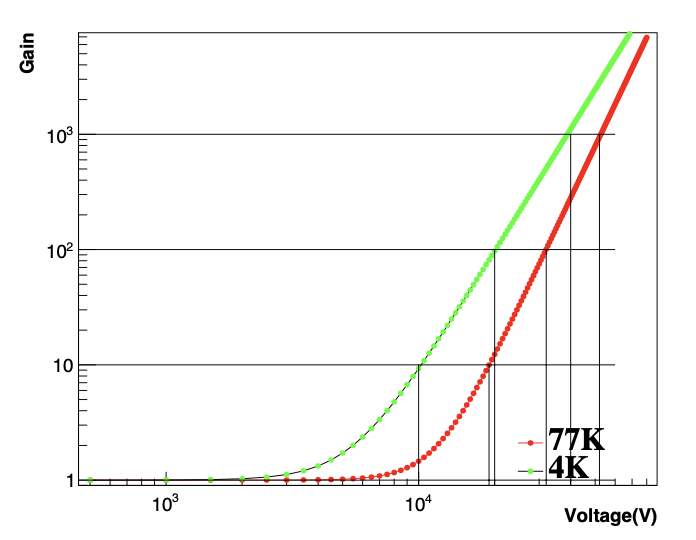
\includegraphics[width=0.4\textwidth]{/Users/yehchihhsiang/Desktop/Chronological_Results/2021-all/Education_Paper/Gain_Factor.png}
  \caption{The gain factor as a function of the voltage under these two temperatures.}
  \label{Gain}
\end{figure}

\begin{figure}[h]
  \centering
  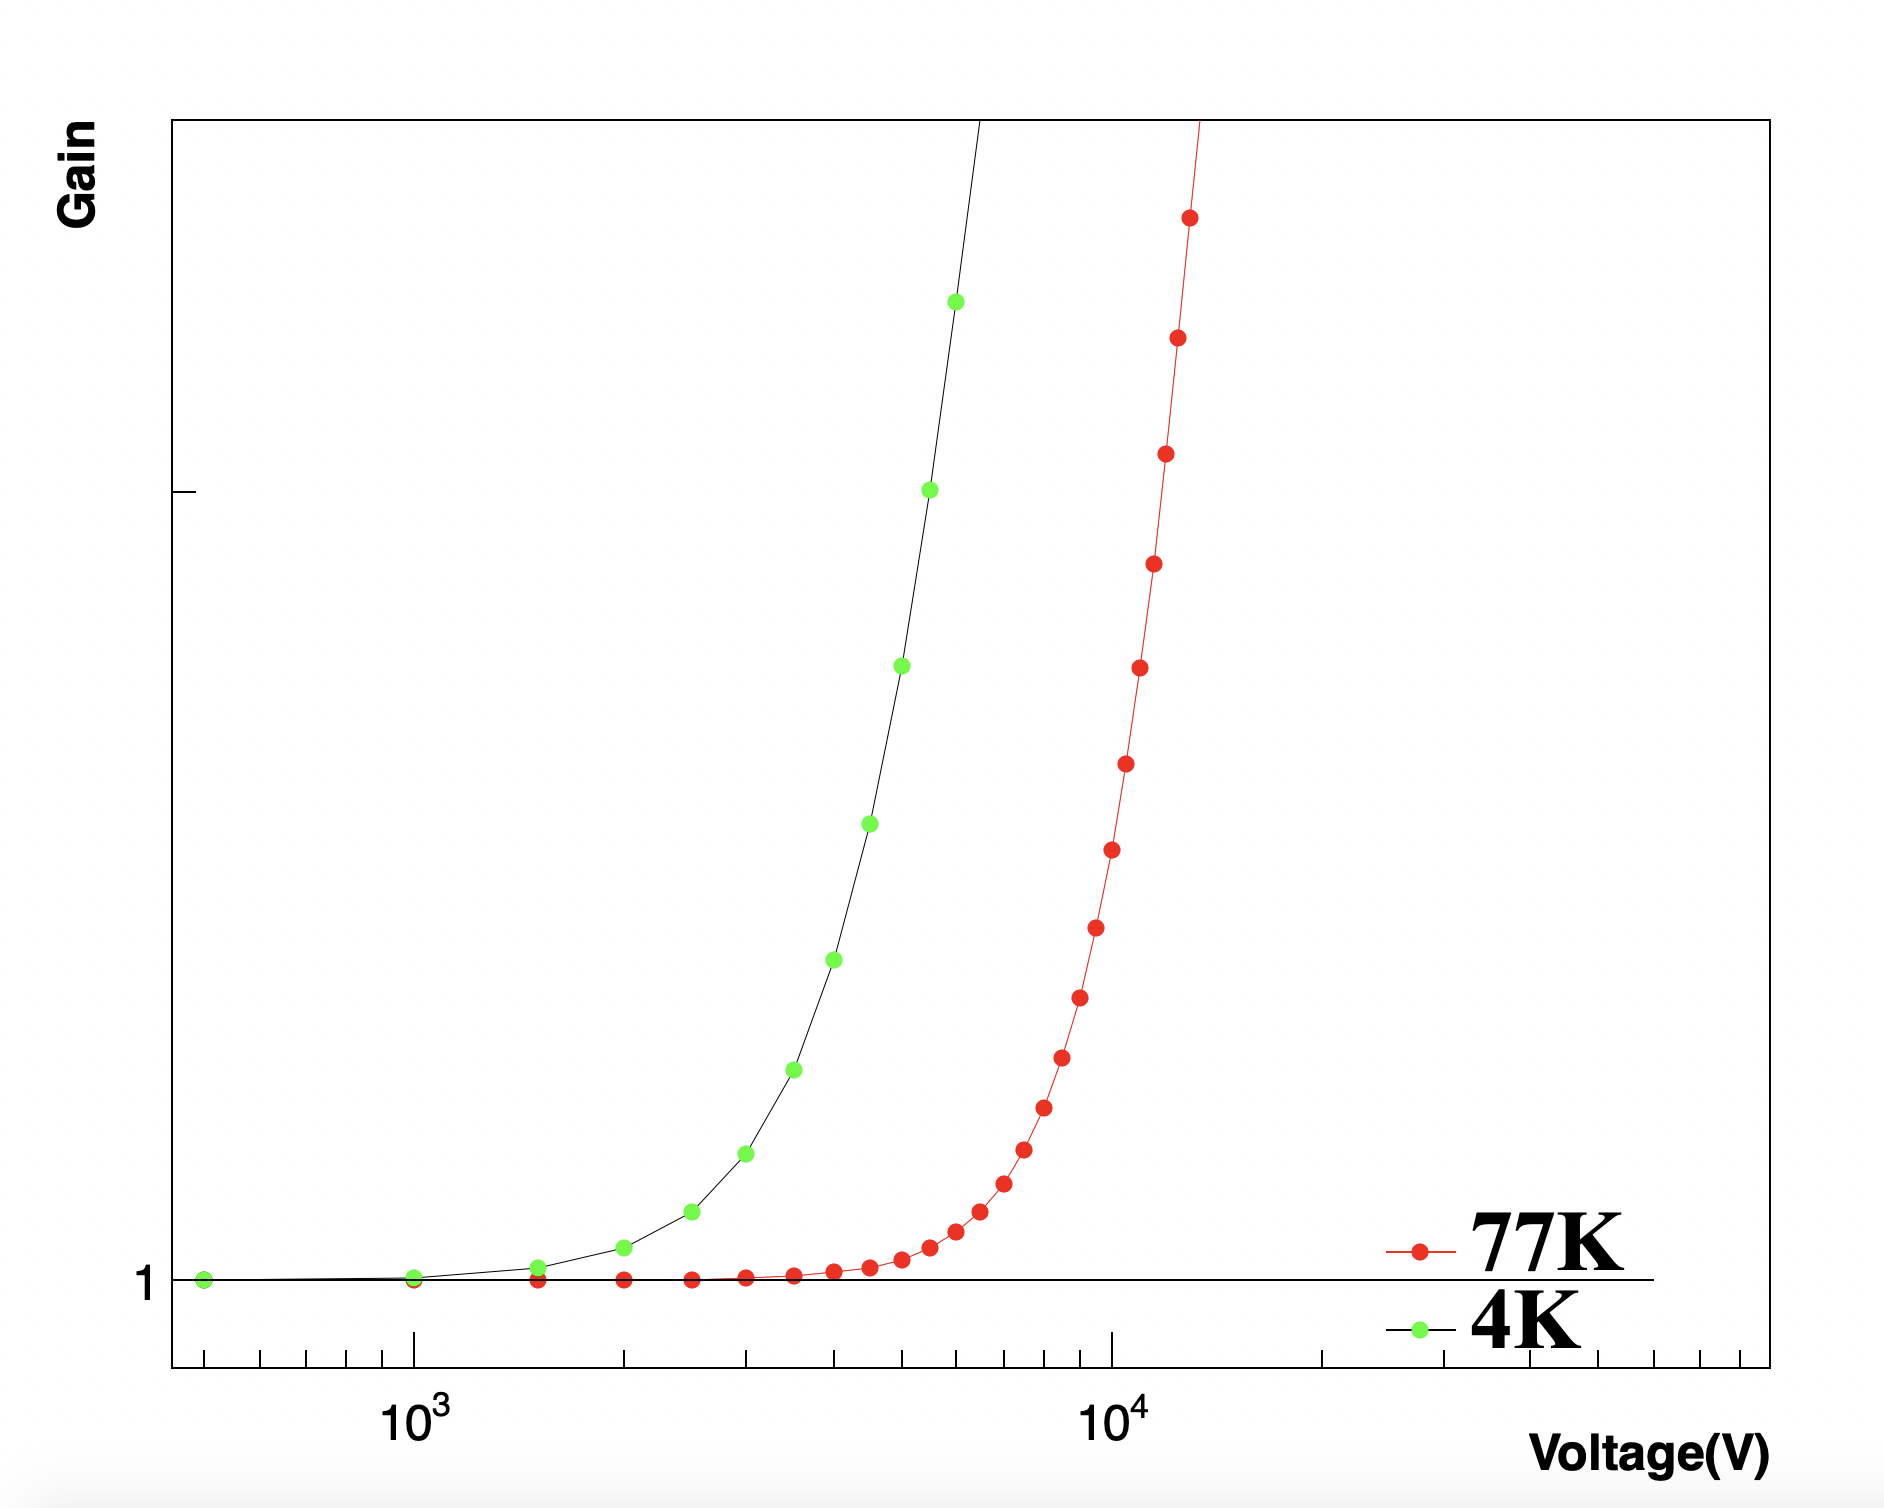
\includegraphics[width=0.4\textwidth]{/Users/yehchihhsiang/Desktop/Chronological_Results/2021-all/Education_Paper/Gain_Zoomin.png}
  \caption{The gain factor as a function of the voltage under these two temperatures.}
  \label{Gain_Zoom}
\end{figure}


\subsection{Electrical Breakdown}
The electrical breakdown can not only alter the electrical properties of the Ge atoms permanently, but also give rise to the grave damage to the crystal, resulting in our effort to grow the available crystal is wrecked. Therefore, the theoretical forecast on the breakdown voltage should be explored ahead of time for preserving our detector from being broken.\\

$E_{ds}$ obeys the following formula\cite{2020AIPA...10b5003Z}:
\begin{equation}\label{EB}
E_{ds}(n,T) = C \times \sqrt[3]{\frac{nT}{2^{n}}}
\end{equation}

C is a constant determined by the experiment, T is the temperature, and n is the gain factor for the amplification of electrical breakdown. If $n>1$, it means that the electrical breakdown is opened up under the high electric field.\\

\begin{figure}[h]
  \centering
  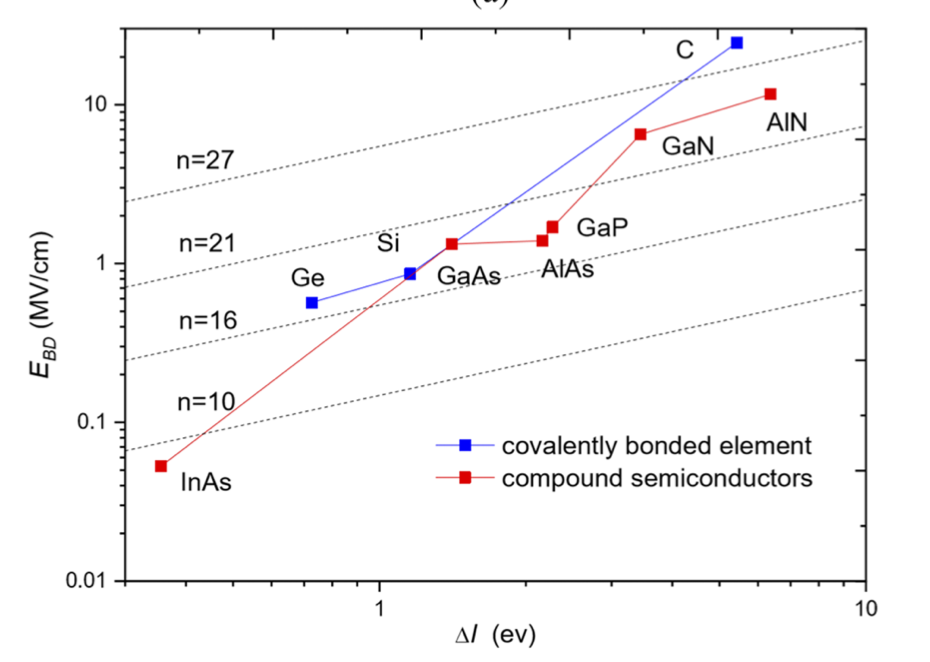
\includegraphics[width=0.4\textwidth]{/Users/yehchihhsiang/Desktop/Chronological_Results/2021-all/Education_Paper/BS_General.png}
  \caption{$\Delta I$ is the bandgap of the material, n is the gain factor, $E_{BD}$ is the electrical strength.}
  \label{BS_General}
\end{figure}

In FIG.\ref{BS_General}\cite{2020AIPA...10b5003Z}, it shows that the breakdown electric field for Ge at 300K is around 0.5(MV/cm) when n equals 16.
With respect to the difference for $E_{ds}$ under two different temperatures, the calculation can be made as follows:
\begin{equation}\label{EB}
E_{ds}(T) = 0.6 \times \sqrt[3]{\frac{1 \times T \times 2^{16}}{16 \times 300 \times 2^{1}}} (MV/cm)
\end{equation}


Since the same gain(Gain$<=$1000) can be accomplished with the lower voltage at 4K as shown in FIG.\ref{Gain}, along with the lower breakdown voltage as depicted above, the $\frac{V}{V_{BD}}$ is introduced to compare how easily the breakdown could happen to the crystal at two temperatures relatively.\\  

As a result of the highest electric field streaming in the detector can dictate the occurrence of the electrical breakdown, the highest electric field under the different voltage should be fully understood. In FIG.\ref{Ex_PPC_Max}, the electric field at r=0.05mm, where is the place on the surface of the contact, is shown as the supreme electric field in the detector under the corresponding voltage applied to the crystal. After using the formula(\ref{EB}) to calculate the breakdown $E_{ds}$ under two temperatures, the matching voltage giving rise to the breakdown electric field can be grabbled by FIG.\ref{Ex_PPC_Max}.\\

In the end, as the voltages resulting in the different gains have already sought in FIG.\ref{Gain}, as well as the research on the voltages for the electrical breakdown under two temperatures are completed, next the comparison of $\frac{V}{V_{BD}}$ can be offered. In TABLE.\ref{Breakdown}, it shows the special pattern: at any gain, all of the ratios at 4K are higher than 77K, meaning that the detector can breakdown more easily at 4K.\\

\begin{figure}[h]
  \centering
  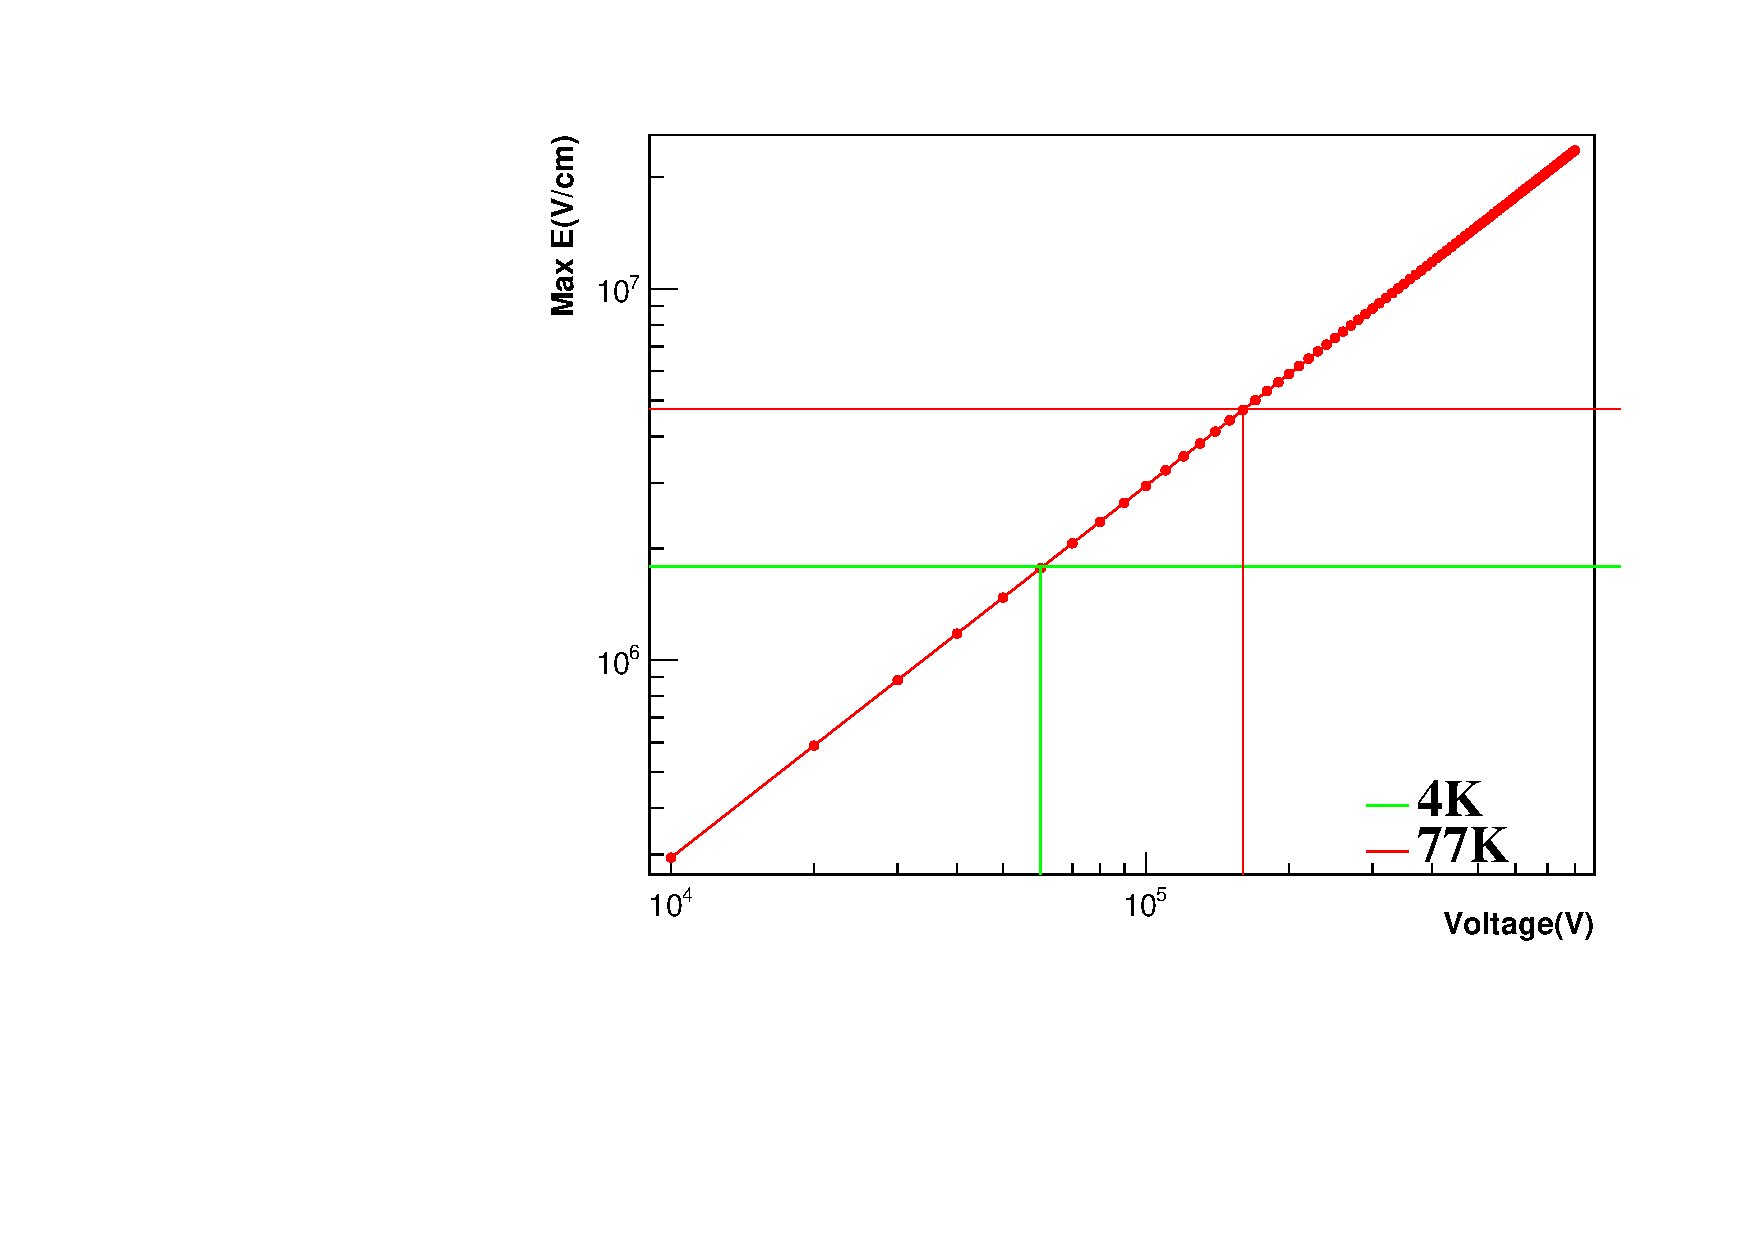
\includegraphics[width=0.4\textwidth]{Ex_PPC_Max.pdf}
  \caption{The max electric field strength as a function of the voltage.}
  \label{Ex_PPC_Max}
\end{figure}

\begin{center}
\begin{table}
 \begin{tabular}{||p{25mm}| p{22mm}| p{22mm}| p{22mm}||} 
 \hline
  & G=10& G=100 &G=1000 \\ 
 \hline\hline
 4K& 0.16667 & 0.333 & 0.6667 \\ [0.5ex] 
 \hline
 77K & 0.095& 0.16& 0.26 \\
  \hline
\end{tabular}
  \caption{$\frac{V}{V_{BD}}$ for a variety of gains under two temperatures.}
  \label{Breakdown}
  \end{table}
\end{center}

%\section{Merits and Predictions for both temperatures}

\section{Conclusion and Dilemma}

\begin{enumerate}
	\item Evidently, if the temperature is lessened to 4K, the leakage currents will be subsided to the level that those contributions to the background can be entirely ignored.
	\item Some strengths aren't always advantages. Even though the same gain can be achieved with the lower voltage at 4K, the crystal should endure the risk of the lower breakdown voltage.
	\item Now the experiment under 4K is anticipated to produce the first version of germanium internal amplification.
\end{enumerate}

\section{To Be Continued....}
Actually, after our literature research incorporating with a load of up-to-date resources, some of the parameters found contracted between different papers. 

\section{Acknowledgement}
Thanks to Prof. Henry Wong at IoPAS on guiding me through the whole studies and providing me a lot of extraordinary advice for the direction of many issues. And thanks to Prof. Dongming on answering me most of the problems originating from the published paper and assisting me see whether the physical concepts I summarize are right.

\bibliographystyle{apsrev4-2} % Tell bibtex which bibliography style to use
\bibliography{GeIANotes_Used}

\end{document}
%%%%%%%%%%%%%%%%%%%%%%%%%%%%%%%%%%%%%%%%%%%%%%%%%%%%%%%%%%%%%%%%%%%%%%%%%%%%%%%%%%%%
The general form and the scheme of the contact leakage current is as follows:
\begin{figure}[h]
    \centering
    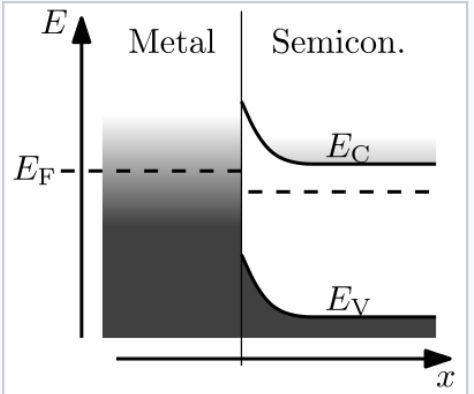
\includegraphics[width=0.25\textwidth]{SHEME/Contact_Leakage_Current.png}
    \caption{Reverse bias: The electrons in the conductive band could jump into the metal band, giving rise to the leakage current}
    \label{fig3}
\end{figure}

\begin{figure}[h]
    \centering
    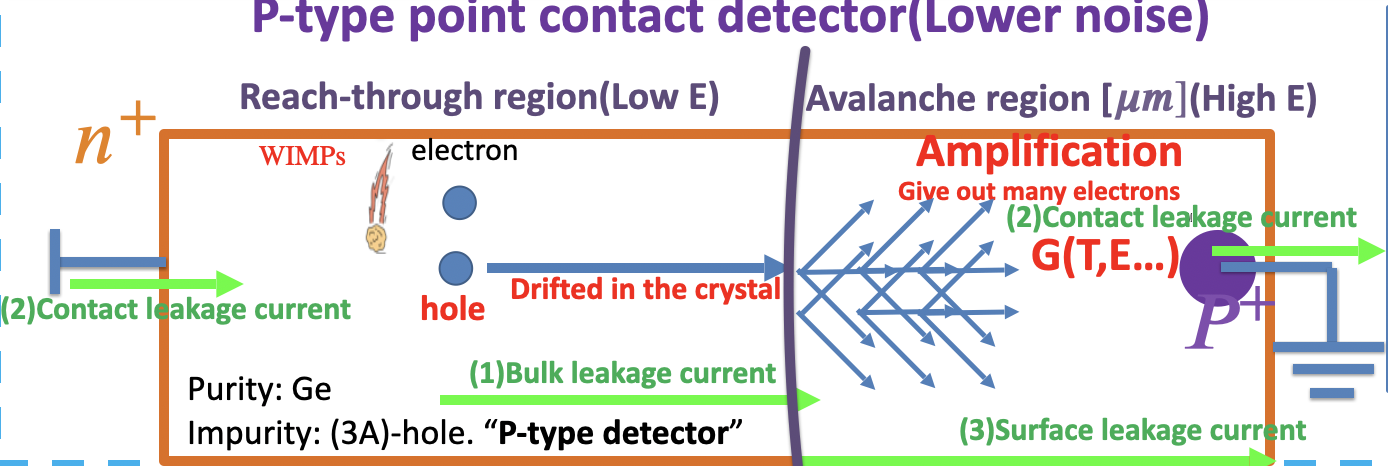
\includegraphics[width=0.5\textwidth]{SHEME/Summary_leakage_ionization_Plot}
    \caption{Reverse bias: The barrier is too high for thermally excited electrons to enter the conduction band from the metal.}
    \label{fig3}
\end{figure}

\begin{figure}[h]
    \centering
    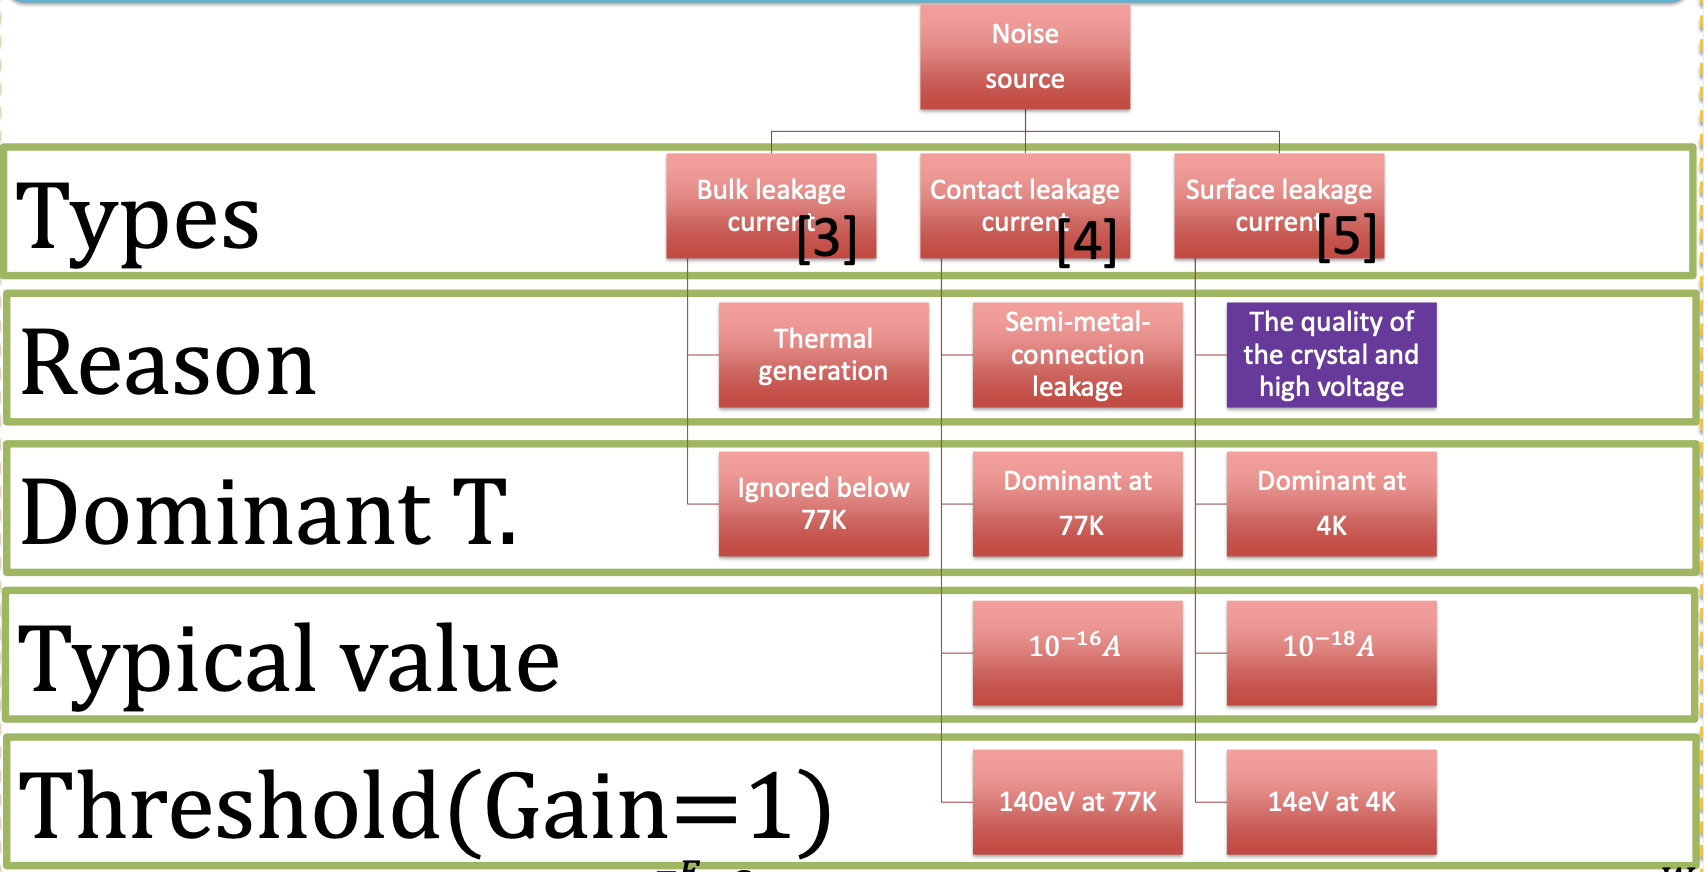
\includegraphics[width=0.5\textwidth]{SHEME/Summary_leakage_ionization}
    \caption{Reverse bias: The barrier is too high for thermally excited electrons to enter the conduction band from the metal.}
    \label{fig3}
\end{figure}

\begin{comment}
An article usually includes an abstract, a concise summary of the work
covered at length in the chief body of the article. 
\begin{description}
\item[Usage]
Secondary publications and information retrieval purposes.
\item[Structure]
You may use the \texttt{description} environment to structure your abstract;
use the optional argument of the \verb+\item+ command to give the category of each item. 
\end{description}
\end{comment}

 \begin{comment}
\author{Second Author}%
 \email{Second.Author@institution.edu}
\affiliation{%
 Authors' institution and/or address\\
 This line break forced with \textbackslash\textbackslash
}%

\collaboration{TEXONO Collaboration}%\noaffiliation

\author{Charlie Author}
 \homepage{http://www.Second.institution.edu/~Charlie.Author}
\affiliation{
 Second institution and/or address\\
 This line break forced% with \\
}%
\affiliation{
 Third institution, the second for Charlie Author
}%
\author{Delta Author}
\affiliation{%
 Authors' institution and/or address\\
 This line break forced with \textbackslash\textbackslash
}%

\subsubsection{Wide text (A level-3 head)}
The \texttt{widetext} environment will make the text the width of the
full page, as on page~\pageref{eq:wideeq}. (Note the use the
\verb+\pageref{#1}+ command to refer to the page number.) 
\paragraph{Note (Fourth-level head is run in)}
The width-changing commands only take effect in two-column formatting. 
There is no effect if text is in a single column.

\subsection{\label{sec:citeref}Citations and References}
A citation in text uses the command \verb+\cite{#1}+ or
\verb+\onlinecite{#1}+ and refers to an entry in the bibliography. 
An entry in the bibliography is a reference to another document.

\subsubsection{Citations}
Because REV\TeX\ uses the \verb+natbib+ package of Patrick Daly, 
the entire repertoire of commands in that package are available for your document;
see the \verb+natbib+ documentation for further details. Please note that
REV\TeX\ requires version 8.31a or later of \verb+natbib+.

\paragraph{Syntax}
The argument of \verb+\cite+ may be a single \emph{key}, 
or may consist of a comma-separated list of keys.
The citation \emph{key} may contain 
letters, numbers, the dash (-) character, or the period (.) character. 
New with natbib 8.3 is an extension to the syntax that allows for 
a star (*) form and two optional arguments on the citation key itself.
The syntax of the \verb+\cite+ command is thus (informally stated)
\begin{quotation}\flushleft\leftskip1em
\verb+\cite+ \verb+{+ \emph{key} \verb+}+, or\\
\verb+\cite+ \verb+{+ \emph{optarg+key} \verb+}+, or\\
\verb+\cite+ \verb+{+ \emph{optarg+key} \verb+,+ \emph{optarg+key}\ldots \verb+}+,
\end{quotation}\noindent
where \emph{optarg+key} signifies 
\begin{quotation}\flushleft\leftskip1em
\emph{key}, or\\
\texttt{*}\emph{key}, or\\
\texttt{[}\emph{pre}\texttt{]}\emph{key}, or\\
\texttt{[}\emph{pre}\texttt{]}\texttt{[}\emph{post}\texttt{]}\emph{key}, or even\\
\texttt{*}\texttt{[}\emph{pre}\texttt{]}\texttt{[}\emph{post}\texttt{]}\emph{key}.
\end{quotation}\noindent
where \emph{pre} and \emph{post} is whatever text you wish to place 
at the beginning and end, respectively, of the bibliographic reference
(see Ref.~[\onlinecite{witten2001}] and the two under Ref.~[\onlinecite{feyn54}]).
(Keep in mind that no automatic space or punctuation is applied.)
It is highly recommended that you put the entire \emph{pre} or \emph{post} portion 
within its own set of braces, for example: 
\verb+\cite+ \verb+{+ \texttt{[} \verb+{+\emph{text}\verb+}+\texttt{]}\emph{key}\verb+}+.
The extra set of braces will keep \LaTeX\ out of trouble if your \emph{text} contains the comma (,) character.

The star (*) modifier to the \emph{key} signifies that the reference is to be 
merged with the previous reference into a single bibliographic entry, 
a common idiom in APS and AIP articles (see below, Ref.~[\onlinecite{epr}]). 
When references are merged in this way, they are separated by a semicolon instead of 
the period (full stop) that would otherwise appear.

\paragraph{Eliding repeated information}
When a reference is merged, some of its fields may be elided: for example, 
when the author matches that of the previous reference, it is omitted. 
If both author and journal match, both are omitted.
If the journal matches, but the author does not, the journal is replaced by \emph{ibid.},
as exemplified by Ref.~[\onlinecite{epr}]. 
These rules embody common editorial practice in APS and AIP journals and will only
be in effect if the markup features of the APS and AIP Bib\TeX\ styles is employed.

\paragraph{The options of the cite command itself}
Please note that optional arguments to the \emph{key} change the reference in the bibliography, 
not the citation in the body of the document. 
For the latter, use the optional arguments of the \verb+\cite+ command itself:
\verb+\cite+ \texttt{*}\allowbreak
\texttt{[}\emph{pre-cite}\texttt{]}\allowbreak
\texttt{[}\emph{post-cite}\texttt{]}\allowbreak
\verb+{+\emph{key-list}\verb+}+.

\subsubsection{Example citations}
By default, citations are numerical\cite{Beutler1994}.
Author-year citations are used when the journal is RMP. 
To give a textual citation, use \verb+\onlinecite{#1}+: 
Refs.~\onlinecite{[][{, and references therein}]witten2001,Bire82}. 
By default, the \texttt{natbib} package automatically sorts your citations into numerical order and ``compresses'' runs of three or more consecutive numerical citations.
REV\TeX\ provides the ability to automatically change the punctuation when switching between journal styles that provide citations in square brackets and those that use a superscript style instead. This is done through the \texttt{citeautoscript} option. For instance, the journal style \texttt{prb} automatically invokes this option because \textit{Physical 
Review B} uses superscript-style citations. The effect is to move the punctuation, which normally comes after a citation in square brackets, to its proper position before the superscript. 
To illustrate, we cite several together 
\cite{[See the explanation of time travel in ]feyn54,*[The classical relativistic treatment of ][ is a relative classic]epr,witten2001,Berman1983,Davies1998,Bire82}, 
and once again in different order (Refs.~\cite{epr,feyn54,Bire82,Berman1983,witten2001,Davies1998}). 
Note that the citations were both compressed and sorted. Futhermore, running this sample file under the \texttt{prb} option will move the punctuation to the correct place.

When the \verb+prb+ class option is used, the \verb+\cite{#1}+ command
displays the reference's number as a superscript rather than in
square brackets. Note that the location of the \verb+\cite{#1}+
command should be adjusted for the reference style: the superscript
references in \verb+prb+ style must appear after punctuation;
otherwise the reference must appear before any punctuation. This
sample was written for the regular (non-\texttt{prb}) citation style.
The command \verb+\onlinecite{#1}+ in the \texttt{prb} style also
displays the reference on the baseline.

\subsubsection{References}
A reference in the bibliography is specified by a \verb+\bibitem{#1}+ command
with the same argument as the \verb+\cite{#1}+ command.
\verb+\bibitem{#1}+ commands may be crafted by hand or, preferably,
generated by Bib\TeX. 
REV\TeX~4.2 includes Bib\TeX\ style files
\verb+apsrev4-2.bst+, \verb+apsrmp4-2.bst+ appropriate for
\textit{Physical Review} and \textit{Reviews of Modern Physics},
respectively.

\subsubsection{Example references}
This sample file employs the \verb+\bibliography+ command, 
which formats the \texttt{\jobname .bbl} file
and specifies which bibliographic databases are to be used by Bib\TeX\ 
(one of these should be by arXiv convention \texttt{\jobname .bib}).
Running Bib\TeX\ (via \texttt{bibtex \jobname}) 
after the first pass of \LaTeX\ produces the file
\texttt{\jobname .bbl} which contains the automatically formatted
\verb+\bibitem+ commands (including extra markup information via
\verb+\bibinfo+ and \verb+\bibfield+ commands). 
If not using Bib\TeX, you will have to create the \verb+thebibiliography+ environment 
and its \verb+\bibitem+ commands by hand.

Numerous examples of the use of the APS bibliographic entry types appear in the bibliography of this sample document.
You can refer to the \texttt{\jobname .bib} file, 
and compare its information to the formatted bibliography itself.

\subsection{Footnotes}%
Footnotes, produced using the \verb+\footnote{#1}+ command, 
usually integrated into the bibliography alongside the other entries.
Numerical citation styles do this%
\footnote{Automatically placing footnotes into the bibliography requires using BibTeX to compile the bibliography.};
author-year citation styles place the footnote at the bottom of the text column.
Note: due to the method used to place footnotes in the bibliography, 
\emph{you must re-run Bib\TeX\ every time you change any of your document's footnotes}. 

\section{Math and Equations}
Inline math may be typeset using the \verb+$+ delimiters. Bold math
symbols may be achieved using the \verb+bm+ package and the
\verb+\bm{#1}+ command it supplies. For instance, a bold $\alpha$ can
be typeset as \verb+$\bm{\alpha}$+ giving $\bm{\alpha}$. Fraktur and
Blackboard (or open face or double struck) characters should be
typeset using the \verb+\mathfrak{#1}+ and \verb+\mathbb{#1}+ commands
respectively. Both are supplied by the \texttt{amssymb} package. For
example, \verb+$\mathbb{R}$+ gives $\mathbb{R}$ and
\verb+$\mathfrak{G}$+ gives $\mathfrak{G}$

In \LaTeX\ there are many different ways to display equations, and a
few preferred ways are noted below. Displayed math will center by
default. Use the class option \verb+fleqn+ to flush equations left.

Below we have numbered single-line equations; this is the most common
type of equation in \textit{Physical Review}:
\begin{eqnarray}
\chi_+(p)\alt{\bf [}2|{\bf p}|(|{\bf p}|+p_z){\bf ]}^{-1/2}
\left(
\begin{array}{c}
|{\bf p}|+p_z\\
px+ip_y
\end{array}\right)\;,
\\
\left\{%
 \openone234567890abc123\alpha\beta\gamma\delta1234556\alpha\beta
 \frac{1\sum^{a}_{b}}{A^2}%
\right\}%
\label{eq:one}.
\end{eqnarray}
Note the open one in Eq.~(\ref{eq:one}).

Not all numbered equations will fit within a narrow column this
way. The equation number will move down automatically if it cannot fit
on the same line with a one-line equation:
\begin{equation}
\left\{
 ab12345678abc123456abcdef\alpha\beta\gamma\delta1234556\alpha\beta
 \frac{1\sum^{a}_{b}}{A^2}%
\right\}.
\end{equation}

When the \verb+\label{#1}+ command is used [cf. input for
Eq.~(\ref{eq:one})], the equation can be referred to in text without
knowing the equation number that \TeX\ will assign to it. Just
use \verb+\ref{#1}+, where \verb+#1+ is the same name that used in
the \verb+\label{#1}+ command.

Unnumbered single-line equations can be typeset
using the \verb+\[+, \verb+\]+ format:
\[g^+g^+ \rightarrow g^+g^+g^+g^+ \dots ~,~~q^+q^+\rightarrow
q^+g^+g^+ \dots ~. \]


\subsection{Multiline equations}

Multiline equations are obtained by using the \verb+eqnarray+
environment.  Use the \verb+\nonumber+ command at the end of each line
to avoid assigning a number:
\begin{eqnarray}
{\cal M}=&&ig_Z^2(4E_1E_2)^{1/2}(l_i^2)^{-1}
\delta_{\sigma_1,-\sigma_2}
(g_{\sigma_2}^e)^2\chi_{-\sigma_2}(p_2)\nonumber\\
&&\times
[\epsilon_jl_i\epsilon_i]_{\sigma_1}\chi_{\sigma_1}(p_1),
\end{eqnarray}
\begin{eqnarray}
\sum \vert M^{\text{viol}}_g \vert ^2&=&g^{2n-4}_S(Q^2)~N^{n-2}
        (N^2-1)\nonumber \\
 & &\times \left( \sum_{i<j}\right)
  \sum_{\text{perm}}
 \frac{1}{S_{12}}
 \frac{1}{S_{12}}
 \sum_\tau c^f_\tau~.
\end{eqnarray}
\textbf{Note:} Do not use \verb+\label{#1}+ on a line of a multiline
equation if \verb+\nonumber+ is also used on that line. Incorrect
cross-referencing will result. Notice the use \verb+\text{#1}+ for
using a Roman font within a math environment.

To set a multiline equation without \emph{any} equation
numbers, use the \verb+\begin{eqnarray*}+,
\verb+\end{eqnarray*}+ format:
\begin{eqnarray*}
\sum \vert M^{\text{viol}}_g \vert ^2&=&g^{2n-4}_S(Q^2)~N^{n-2}
        (N^2-1)\\
 & &\times \left( \sum_{i<j}\right)
 \left(
  \sum_{\text{perm}}\frac{1}{S_{12}S_{23}S_{n1}}
 \right)
 \frac{1}{S_{12}}~.
\end{eqnarray*}

To obtain numbers not normally produced by the automatic numbering,
use the \verb+\tag{#1}+ command, where \verb+#1+ is the desired
equation number. For example, to get an equation number of
(\ref{eq:mynum}),
\begin{equation}
g^+g^+ \rightarrow g^+g^+g^+g^+ \dots ~,~~q^+q^+\rightarrow
q^+g^+g^+ \dots ~. \tag{2.6$'$}\label{eq:mynum}
\end{equation}

\paragraph{A few notes on \texttt{tag}s} 
\verb+\tag{#1}+ requires the \texttt{amsmath} package. 
Place the \verb+\tag{#1}+ command before the \verb+\label{#1}+, if any. 
The numbering produced by \verb+\tag{#1}+ \textit{does not affect} 
the automatic numbering in REV\TeX; 
therefore, the number must be known ahead of time, 
and it must be manually adjusted if other equations are added. 
\verb+\tag{#1}+ works with both single-line and multiline equations. 
\verb+\tag{#1}+ should only be used in exceptional cases---%
do not use it to number many equations in your paper. 
Please note that this feature of the \texttt{amsmath} package
is \emph{not} compatible with the \texttt{hyperref} (6.77u) package.

Enclosing display math within
\verb+\begin{subequations}+ and \verb+\end{subequations}+ will produce
a set of equations that are labeled with letters, as shown in
Eqs.~(\ref{subeq:1}) and (\ref{subeq:2}) below.
You may include any number of single-line and multiline equations,
although it is probably not a good idea to follow one display math
directly after another.
\begin{subequations}
\label{eq:whole}
\begin{eqnarray}
{\cal M}=&&ig_Z^2(4E_1E_2)^{1/2}(l_i^2)^{-1}
(g_{\sigma_2}^e)^2\chi_{-\sigma_2}(p_2)\nonumber\\
&&\times
[\epsilon_i]_{\sigma_1}\chi_{\sigma_1}(p_1).\label{subeq:2}
\end{eqnarray}
\begin{equation}
\left\{
 abc123456abcdef\alpha\beta\gamma\delta1234556\alpha\beta
 \frac{1\sum^{a}_{b}}{A^2}
\right\},\label{subeq:1}
\end{equation}
\end{subequations}
Giving a \verb+\label{#1}+ command directly after the \verb+\begin{subequations}+, 
allows you to reference all the equations in the \texttt{subequations} environment. 
For example, the equations in the preceding subequations environment were
Eqs.~(\ref{eq:whole}).

\subsubsection{Wide equations}
The equation that follows is set in a wide format, i.e., it spans the full page. 
The wide format is reserved for long equations
that cannot easily be set in a single column:
\begin{widetext}
\begin{equation}
{\cal R}^{(\text{d})}=
 g_{\sigma_2}^e
 \left(
   \frac{[\Gamma^Z(3,21)]_{\sigma_1}}{Q_{12}^2-M_W^2}
  +\frac{[\Gamma^Z(13,2)]_{\sigma_1}}{Q_{13}^2-M_W^2}
 \right)
 + x_WQ_e
 \left(
   \frac{[\Gamma^\gamma(3,21)]_{\sigma_1}}{Q_{12}^2-M_W^2}
  +\frac{[\Gamma^\gamma(13,2)]_{\sigma_1}}{Q_{13}^2-M_W^2}
 \right)\;. 
 \label{eq:wideeq}
\end{equation}
\end{widetext}
This is typed to show how the output appears in wide format.
(Incidentally, since there is no blank line between the \texttt{equation} environment above 
and the start of this paragraph, this paragraph is not indented.)

\section{Cross-referencing}
REV\TeX{} will automatically number such things as
sections, footnotes, equations, figure captions, and table captions. 
In order to reference them in text, use the
\verb+\label{#1}+ and \verb+\ref{#1}+ commands. 
To reference a particular page, use the \verb+\pageref{#1}+ command.

The \verb+\label{#1}+ should appear 
within the section heading, 
within the footnote text, 
within the equation, or 
within the table or figure caption. 
The \verb+\ref{#1}+ command
is used in text at the point where the reference is to be displayed.  
Some examples: Section~\ref{sec:level1} on page~\pageref{sec:level1},
Table~\ref{tab:table1},%
\begin{table}[b]%The best place to locate the table environment is directly after its first reference in text
\caption{\label{tab:table1}%
A table that fits into a single column of a two-column layout. 
Note that REV\TeX~4 adjusts the intercolumn spacing so that the table fills the
entire width of the column. Table captions are numbered
automatically. 
This table illustrates left-, center-, decimal- and right-aligned columns,
along with the use of the \texttt{ruledtabular} environment which sets the 
Scotch (double) rules above and below the alignment, per APS style.
}
\begin{ruledtabular}
\begin{tabular}{lcdr}
\textrm{Left\footnote{Note a.}}&
\textrm{Centered\footnote{Note b.}}&
\multicolumn{1}{c}{\textrm{Decimal}}&
\textrm{Right}\\
\colrule
1 & 2 & 3.001 & 4\\
10 & 20 & 30 & 40\\
100 & 200 & 300.0 & 400\\
\end{tabular}
\end{ruledtabular}
\end{table}
and Fig.~\ref{fig:epsart}.%
\begin{figure}[b]
\includegraphics{fig_1}% Here is how to import EPS art
\caption{\label{fig:epsart} A figure caption. The figure captions are
automatically numbered.}
\end{figure}

\section{Floats: Figures, Tables, Videos, etc.}
Figures and tables are usually allowed to ``float'', which means that their
placement is determined by \LaTeX, while the document is being typeset. 

Use the \texttt{figure} environment for a figure, the \texttt{table} environment for a table.
In each case, use the \verb+\caption+ command within to give the text of the
figure or table caption along with the \verb+\label+ command to provide
a key for referring to this figure or table.
The typical content of a figure is an image of some kind; 
that of a table is an alignment.%
\begin{figure*}
\includegraphics{fig_2}% Here is how to import EPS art
\caption{\label{fig:wide}Use the figure* environment to get a wide
figure that spans the page in \texttt{twocolumn} formatting.}
\end{figure*}
\begin{table*}
\caption{\label{tab:table3}This is a wide table that spans the full page
width in a two-column layout. It is formatted using the
\texttt{table*} environment. It also demonstates the use of
\textbackslash\texttt{multicolumn} in rows with entries that span
more than one column.}
\begin{ruledtabular}
\begin{tabular}{ccccc}
 &\multicolumn{2}{c}{$D_{4h}^1$}&\multicolumn{2}{c}{$D_{4h}^5$}\\
 Ion&1st alternative&2nd alternative&lst alternative
&2nd alternative\\ \hline
 K&$(2e)+(2f)$&$(4i)$ &$(2c)+(2d)$&$(4f)$ \\
 Mn&$(2g)$\footnote{The $z$ parameter of these positions is $z\sim\frac{1}{4}$.}
 &$(a)+(b)+(c)+(d)$&$(4e)$&$(2a)+(2b)$\\
 Cl&$(a)+(b)+(c)+(d)$&$(2g)$\footnotemark[1]
 &$(4e)^{\text{a}}$\\
 He&$(8r)^{\text{a}}$&$(4j)^{\text{a}}$&$(4g)^{\text{a}}$\\
 Ag& &$(4k)^{\text{a}}$& &$(4h)^{\text{a}}$\\
\end{tabular}
\end{ruledtabular}
\end{table*}

Insert an image using either the \texttt{graphics} or
\texttt{graphix} packages, which define the \verb+\includegraphics{#1}+ command.
(The two packages differ in respect of the optional arguments 
used to specify the orientation, scaling, and translation of the image.) 
To create an alignment, use the \texttt{tabular} environment. 

The best place to locate the \texttt{figure} or \texttt{table} environment
is immediately following its first reference in text; this sample document
illustrates this practice for Fig.~\ref{fig:epsart}, which
shows a figure that is small enough to fit in a single column. 

In exceptional cases, you will need to move the float earlier in the document, as was done
with Table~\ref{tab:table3}: \LaTeX's float placement algorithms need to know
about a full-page-width float earlier. 

Fig.~\ref{fig:wide}
has content that is too wide for a single column,
so the \texttt{figure*} environment has been used.%
\begin{table}[b]
\caption{\label{tab:table4}%
Numbers in columns Three--Five are aligned with the ``d'' column specifier 
(requires the \texttt{dcolumn} package). 
Non-numeric entries (those entries without a ``.'') in a ``d'' column are aligned on the decimal point. 
Use the ``D'' specifier for more complex layouts. }
\begin{ruledtabular}
\begin{tabular}{ccddd}
One&Two&
\multicolumn{1}{c}{\textrm{Three}}&
\multicolumn{1}{c}{\textrm{Four}}&
\multicolumn{1}{c}{\textrm{Five}}\\
%\mbox{Three}&\mbox{Four}&\mbox{Five}\\
\hline
one&two&\mbox{three}&\mbox{four}&\mbox{five}\\
He&2& 2.77234 & 45672. & 0.69 \\
C\footnote{Some tables require footnotes.}
  &C\footnote{Some tables need more than one footnote.}
  & 12537.64 & 37.66345 & 86.37 \\
\end{tabular}
\end{ruledtabular}
\end{table}

The content of a table is typically a \texttt{tabular} environment, 
giving rows of type in aligned columns. 
Column entries separated by \verb+&+'s, and 
each row ends with \textbackslash\textbackslash. 
The required argument for the \texttt{tabular} environment
specifies how data are aligned in the columns. 
For instance, entries may be centered, left-justified, right-justified, aligned on a decimal
point. 
Extra column-spacing may be be specified as well, 
although REV\TeX~4 sets this spacing so that the columns fill the width of the
table. Horizontal rules are typeset using the \verb+\hline+
command. The doubled (or Scotch) rules that appear at the top and
bottom of a table can be achieved enclosing the \texttt{tabular}
environment within a \texttt{ruledtabular} environment. Rows whose
columns span multiple columns can be typeset using the
\verb+\multicolumn{#1}{#2}{#3}+ command (for example, see the first
row of Table~\ref{tab:table3}).%

Tables~\ref{tab:table1}, \ref{tab:table3}, \ref{tab:table4}, and \ref{tab:table2}%
\begin{table}[b]
\caption{\label{tab:table2}
A table with numerous columns that still fits into a single column. 
Here, several entries share the same footnote. 
Inspect the \LaTeX\ input for this table to see exactly how it is done.}
\begin{ruledtabular}
\begin{tabular}{cccccccc}
 &$r_c$ (\AA)&$r_0$ (\AA)&$\kappa r_0$&
 &$r_c$ (\AA) &$r_0$ (\AA)&$\kappa r_0$\\
\hline
Cu& 0.800 & 14.10 & 2.550 &Sn\footnotemark[1]
& 0.680 & 1.870 & 3.700 \\
Ag& 0.990 & 15.90 & 2.710 &Pb\footnotemark[2]
& 0.450 & 1.930 & 3.760 \\
Au& 1.150 & 15.90 & 2.710 &Ca\footnotemark[3]
& 0.750 & 2.170 & 3.560 \\
Mg& 0.490 & 17.60 & 3.200 &Sr\footnotemark[4]
& 0.900 & 2.370 & 3.720 \\
Zn& 0.300 & 15.20 & 2.970 &Li\footnotemark[2]
& 0.380 & 1.730 & 2.830 \\
Cd& 0.530 & 17.10 & 3.160 &Na\footnotemark[5]
& 0.760 & 2.110 & 3.120 \\
Hg& 0.550 & 17.80 & 3.220 &K\footnotemark[5]
&  1.120 & 2.620 & 3.480 \\
Al& 0.230 & 15.80 & 3.240 &Rb\footnotemark[3]
& 1.330 & 2.800 & 3.590 \\
Ga& 0.310 & 16.70 & 3.330 &Cs\footnotemark[4]
& 1.420 & 3.030 & 3.740 \\
In& 0.460 & 18.40 & 3.500 &Ba\footnotemark[5]
& 0.960 & 2.460 & 3.780 \\
Tl& 0.480 & 18.90 & 3.550 & & & & \\
\end{tabular}
\end{ruledtabular}
\footnotetext[1]{Here's the first, from Ref.~\onlinecite{feyn54}.}
\footnotetext[2]{Here's the second.}
\footnotetext[3]{Here's the third.}
\footnotetext[4]{Here's the fourth.}
\footnotetext[5]{And etc.}
\end{table}
show various effects.
A table that fits in a single column employs the \texttt{table}
environment. 
Table~\ref{tab:table3} is a wide table, set with the \texttt{table*} environment. 
Long tables may need to break across pages. 
The most straightforward way to accomplish this is to specify
the \verb+[H]+ float placement on the \texttt{table} or
\texttt{table*} environment. 
However, the \LaTeXe\ package \texttt{longtable} allows headers and footers to be specified for each page of the table. 
A simple example of the use of \texttt{longtable} can be found
in the file \texttt{summary.tex} that is included with the REV\TeX~4
distribution.

There are two methods for setting footnotes within a table (these
footnotes will be displayed directly below the table rather than at
the bottom of the page or in the bibliography). The easiest
and preferred method is just to use the \verb+\footnote{#1}+
command. This will automatically enumerate the footnotes with
lowercase roman letters. However, it is sometimes necessary to have
multiple entries in the table share the same footnote. In this case,
there is no choice but to manually create the footnotes using
\verb+\footnotemark[#1]+ and \verb+\footnotetext[#1]{#2}+.
\texttt{\#1} is a numeric value. Each time the same value for
\texttt{\#1} is used, the same mark is produced in the table. The
\verb+\footnotetext[#1]{#2}+ commands are placed after the \texttt{tabular}
environment. Examine the \LaTeX\ source and output for
Tables~\ref{tab:table1} and \ref{tab:table2}
for examples.

Video~\ref{vid:PRSTPER.4.010101} 
illustrates several features new with REV\TeX4.2,
starting with the \texttt{video} environment, which is in the same category with
\texttt{figure} and \texttt{table}.%
\begin{video}
\href{http://prst-per.aps.org/multimedia/PRSTPER/v4/i1/e010101/e010101_vid1a.mpg}{\includegraphics{vid_1a}}%
 \quad
\href{http://prst-per.aps.org/multimedia/PRSTPER/v4/i1/e010101/e010101_vid1b.mpg}{\includegraphics{vid_1b}}
 \setfloatlink{http://link.aps.org/multimedia/PRSTPER/v4/i1/e010101}%
 \caption{\label{vid:PRSTPER.4.010101}%
  Students explain their initial idea about Newton's third law to a teaching assistant. 
  Clip (a): same force.
  Clip (b): move backwards.
 }%
\end{video}
The \verb+\setfloatlink+ command causes the title of the video to be a hyperlink to the
indicated URL; it may be used with any environment that takes the \verb+\caption+
command.
The \verb+\href+ command has the same significance as it does in the context of
the \texttt{hyperref} package: the second argument is a piece of text to be 
typeset in your document; the first is its hyperlink, a URL.

\textit{Physical Review} style requires that the initial citation of
figures or tables be in numerical order in text, so don't cite
Fig.~\ref{fig:wide} until Fig.~\ref{fig:epsart} has been cited.

\begin{acknowledgments}
We wish to acknowledge the support of the author community in using
REV\TeX{}, offering suggestions and encouragement, testing new versions,
\dots.
\end{acknowledgments}

\appendix

\section{Appendixes}

To start the appendixes, use the \verb+\appendix+ command.
This signals that all following section commands refer to appendixes
instead of regular sections. Therefore, the \verb+\appendix+ command
should be used only once---to setup the section commands to act as
appendixes. Thereafter normal section commands are used. The heading
for a section can be left empty. For example,
\begin{verbatim}
\appendix
\section{}
\end{verbatim}
will produce an appendix heading that says ``APPENDIX A'' and
\begin{verbatim}
\appendix
\section{Background}
\end{verbatim}
will produce an appendix heading that says ``APPENDIX A: BACKGROUND''
(note that the colon is set automatically).

If there is only one appendix, then the letter ``A'' should not
appear. This is suppressed by using the star version of the appendix
command (\verb+\appendix*+ in the place of \verb+\appendix+).

\section{A little more on appendixes}

Observe that this appendix was started by using
\begin{verbatim}
\section{A little more on appendixes}
\end{verbatim}

Note the equation number in an appendix:
\begin{equation}
E=mc^2.
\end{equation}

\subsection{\label{app:subsec}A subsection in an appendix}

You can use a subsection or subsubsection in an appendix. Note the
numbering: we are now in Appendix~\ref{app:subsec}.

Note the equation numbers in this appendix, produced with the
subequations environment:
\begin{subequations}
\begin{eqnarray}
E&=&mc, \label{appa}
\\
E&=&mc^2, \label{appb}
\\
E&\agt& mc^3. \label{appc}
\end{eqnarray}
\end{subequations}
They turn out to be Eqs.~(\ref{appa}), (\ref{appb}), and (\ref{appc}).

% The \nocite command causes all entries in a bibliography to be printed out
% whether or not they are actually referenced in the text. This is appropriate
% for the sample file to show the different styles of references, but authors
% most likely will not want to use it.
\nocite{*}

\bibliography{apssamp}% Produces the bibliography via BibTeX.


Weakly interacting massive particle(WIMP), which is the most promising candidate for dark matter, is the delicious prey in a variety of facets that many experiments are hunting for. To explore the probable signal, a bunch of approaches including the direct-detection experiments, are now trying to extend their capability of measuring the broader range of mass of dark matter. To extend the possibility of investigating in the lower-mass region for WIMP, the ultra-low threshold detector should be fabricated. In this project, we have an attempt to dissect the solid-state physics process happening in the detector to see how to improve the performance of it theoretically and recognize the limits of the detector with the controllable parameters provided. \\

It is related to the conductivity of the electron in the crystal. In the paper\cite{7}, basically, all of the important information is included.\\

From (\ref{Mobility_Sum}), which is used to summarize the mobility from the different contribution  as follows:
		\begin{equation}\label{Mobility_Sum}
  	 	 \frac{1}{\mu}=  \frac{1}{\mu_{1}} + \frac{1}{\mu_{2}} + \frac{1}{\mu_{3}} + ....
  		  \end{equation}
The intriguing thing is that, "the smaller the individual mobility, the higher the importance that is".\\
 
From our research, actually, there are two eventful scattering processes that should be taken int account, which are the acoustic phonon scattering, as well as the neutral impurity scattering.  In Fig.\ref{Phonon_Scattering_Mobility}, the empirical formula is consider in our studies, if the temperature becomes smaller, the mobility will grow higher, resulting in the less important tendency. Oppositely, since the neutral impurity isn't affected by the temperature too much, the $2 \times 10^{15} cm^{-3}$ is assumed to be the neutral impurity level for both temperatures in Fig.\ref{Neutral_Impurity_Mobility}.\\ 

Comparing between these two figures, the conclusion can be made that at 77K. the acoustic phonon scattering is the dominant one(the smaller one), but at 4K, the neutral impurity scattering is the dominant one. 

\begin{figure}[h]
  \centering
  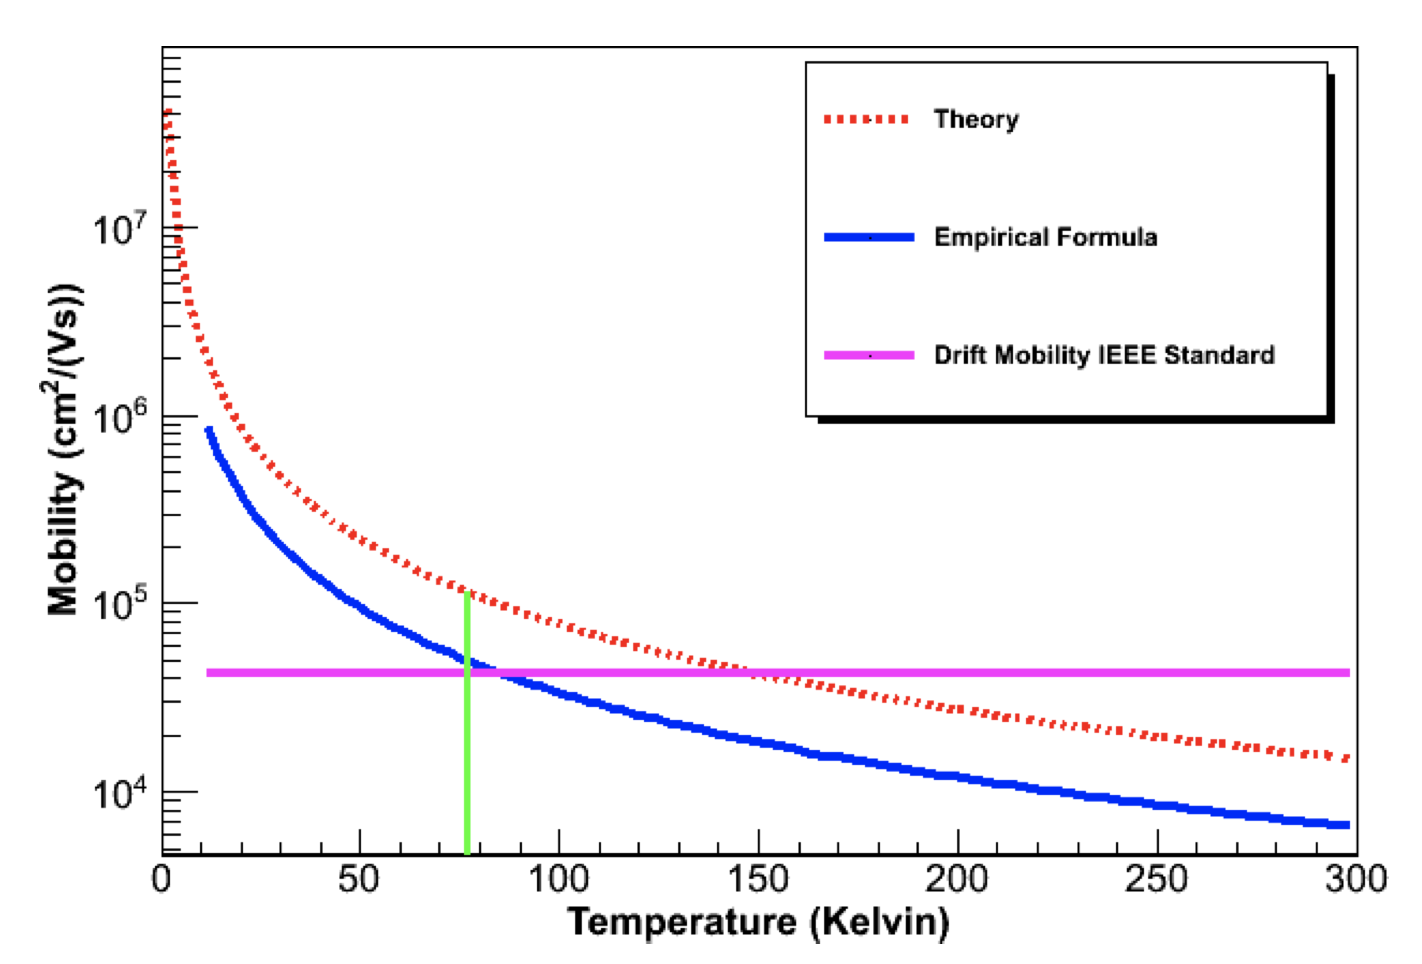
\includegraphics[width=0.35\textwidth]{SHEME/Phonon_Scattering_Mobility.png}
  \caption{The mobility due to acoustic phonon scattering as a function of temperature.}
  \label{Phonon_Scattering_Mobility}
\end{figure}

\begin{figure}[h]
  \centering
  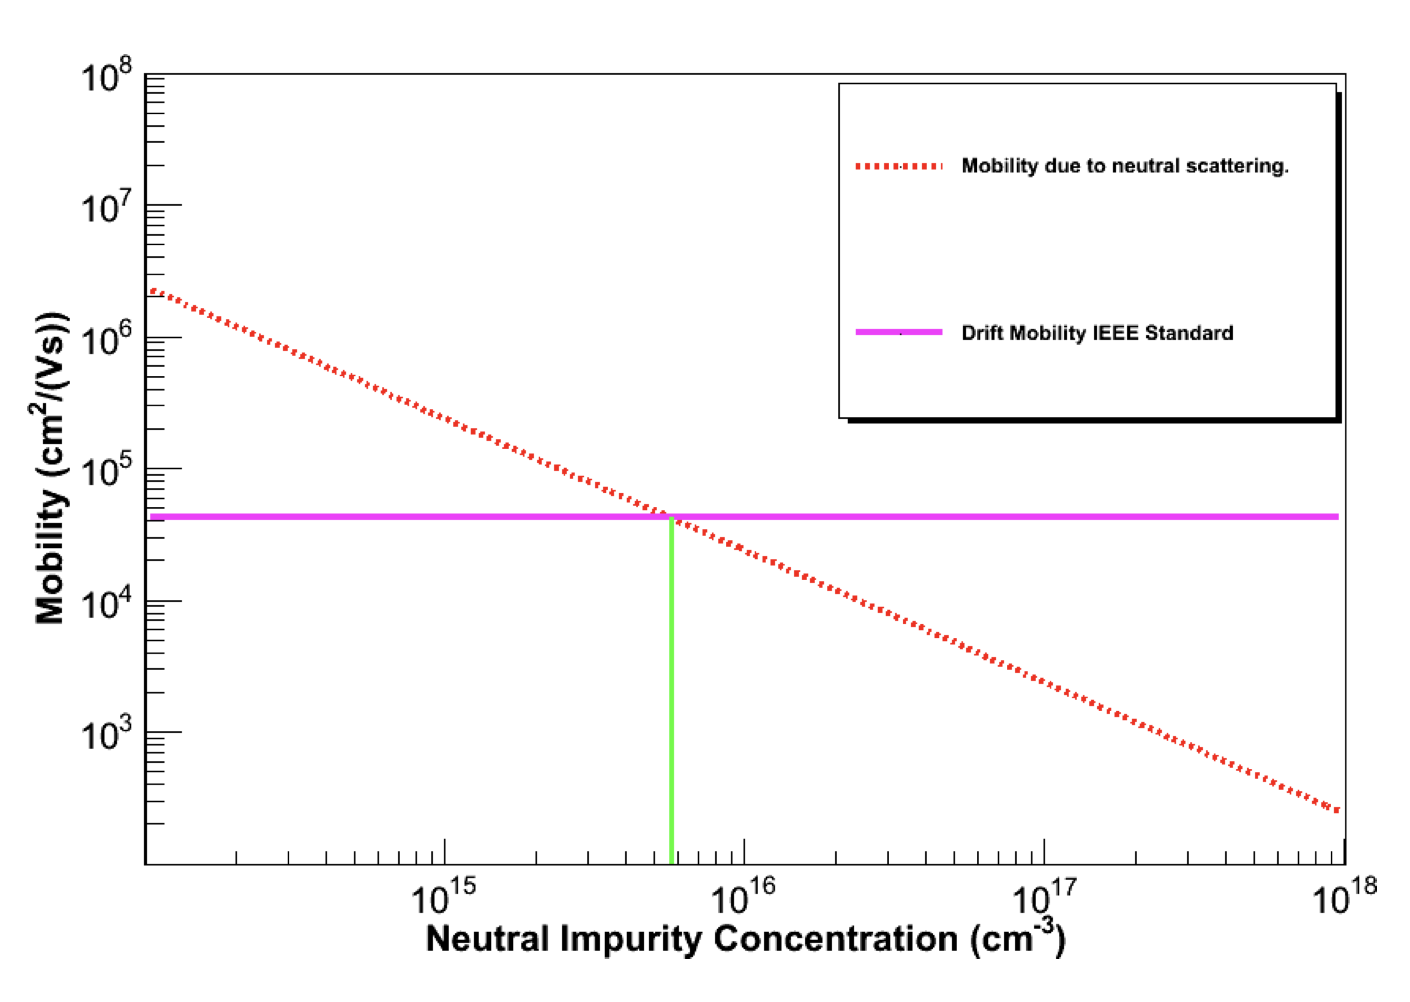
\includegraphics[width=0.35\textwidth]{SHEME/Neutral_Impurity_Mobility.png}
  \caption{The mobility due to neutral impurity scattering calculated by Erginsoy’s model as a function of neutral impurity concentration.}
  \label{Neutral_Impurity_Mobility}
\end{figure}

\begin{center}\label{}
 \begin{tabular}{||p{25mm}| p{22mm}| p{22mm}| p{22mm}||} 
 \hline
 Type & Bulk& Contact & Surface \\ 
 \hline\hline
 Reason&Thermal generation & Semi-metal-connection leakage & The quality of the crystal and high voltage \\ [0.5ex] 
 \hline
 Dominant T. & Ignored below 77K & Dominant at 77K & Dominant at 4K \\
 \hline
 Typical value & Ignored & $10^{-13}A$ & $<10^{-40}A$ \\
 \hline
 Threshold (Gain=1) & No & 140eV at 77K  & 14eV at 4K\\
 \hline
 \hline
\end{tabular}
\end{center}
Since the bandgap between the conductive band and the valance band is around 0.68eV, the energy stockpiled in the capacitance(detector) should be around this number for letting the electrons in the valance band have the sufficient energy to hop to the conductive band, bringing about the breakdown occurring in the crystal.\\

The simple estimation can be compiled with the calculation demonstrated as follows:
\begin{equation}\label{bulk_leakage_current}
u = \frac{1}{2} \times \epsilon_{r} \epsilon_{0}  \times E^{2}\\
\end{equation}

u is the energy stored in the capacitance, and $\epsilon_{r}$ is the relative permittivity, differing between the different material. $\epsilon_{r}$ is the vacuum permittivity, and E is the electric field distributing in the crystal.\\

After the substitutions for those parameters with the authentic numbers from our experiment, the calculations can be generated as follows:
\begin{equation}\label{bulk_leakage_current}
  \frac{1}{2} \times 16 \times (8.8 \times 10^{-12} ) \times E^{2} = 0.68eV
\end{equation}

In the end, the final result for the scale of E is around E(MV/cm) for the electrical breakdown. To compare between the experimental values on the scale of electrical breakdown at varying temperatures, $E_{ds}$, which is employed to delineate the electric field strength at which the breakdown occurs, would be investigated. \\

Basically, the breakdown electric field for the crystal under 77K is three times higher than the case under 4K. Since there is no exact number of the breakdown electric field for Ge, the small assumption, which is that the breakdown electric field is 1(MV/cm) at 77K and is $\frac{1}{2.68}$(MV/cm) at 4K, is made for comparing the degree of difficulty on the breakdown at both temperatures fairly.\\

From the definition of electrical mobility\cite{Mei:2019usy}. which is as follows:\par
\begin{equation}
\label{MFP}
\mu = \frac{\mu_{0}}{1 + \frac{\mu_{0}E}{V_{sat}}}
\end{equation}

where $\mu_{0}$, which is set as the number given in the TABLE.\ref{The_mobilities} from the report delivered by Prof. Dongming(2019-07-17), is the mobility of the charge carrier at zero field, $E$ is the electric field applied to the crystal., and $V_{sat}$ is the saturation velocity of the electron, which can be inferred by the following formula\cite{Mei:2019usy}:\\

\begin{center}
\begin{table}
 \begin{tabular}{||p{25mm}| p{22mm}| p{22mm}| p{22mm}||} 
 \hline
  $\mu_{0}(cm^{2}/Vs)$& Electron& Hole \\ 
 \hline\hline
 4K& $10^{6}$ & $10^{6}$  \\ [0.5ex] 
 \hline
 77K & $3.6 \times 10^{4}$ & $4.2 \times 10^{4}$\\
  \hline
\end{tabular}
  \caption{The mobilities of the electron and hole at zero field under two temperatures.}
  \label{The_mobilities}
  \end{table}
\end{center}

\begin{equation}
\label{MFP}
V_{sat} = \frac{V_{sat}^{300K}}{1-A_{\nu}+A_{\nu}(\frac{T}{300})}
\end{equation}

where $A_{\nu}$ is 0.55 for electrons at 300K and is 0.61 for holes at 300K. The $V_{sat}$ under any temperature can be figured out with this formula.\par

\end{comment}

%
% ****** End of file apssamp.tex ******
